%% This is "sig-alternate.tex" V2.1 April 2013
% This file should be compiled with V2.5 of "sig-alternate.cls" May 2012
%
% This example file demonstrates the use of the 'sig-alternate.cls'
% V2.5 LaTeX2e document class file. It is for those submitting
% articles to ACM Conference Proceedings WHO DO NOT WISH TO
% STRICTLY ADHERE TO THE SIGS (PUBS-BOARD-ENDORSED) STYLE.
% The 'sig-alternate.cls' file will produce a similar-looking,
% albeit, 'tighter' paper resulting in, invariably, fewer pages.
%
% ----------------------------------------------------------------------------------------------------------------
% This .tex file (and associated .cls V2.5) produces:
%       1) The Permission Statement
%       2) The Conference (location) Info information
%       3) The Copyright Line with ACM data
%       4) NO page numbers
%
% as against the acm_proc_article-sp.cls file which
% DOES NOT produce 1) thru' 3) above.
%
% Using 'sig-alternate.cls' you have control, however, from within
% the source .tex file, over both the CopyrightYear
% (defaulted to 200X) and the ACM Copyright Data
% (defaulted to X-XXXXX-XX-X/XX/XX).
% e.g.
% \CopyrightYear{2007} will cause 2007 to appear in the copyright line.
% \crdata{0-12345-67-8/90/12} will cause 0-12345-67-8/90/12 to appear in the copyright line.
%
% ---------------------------------------------------------------------------------------------------------------
% This .tex source is an example which *does* use
% the .bib file (from which the .bbl file % is produced).
% REMEMBER HOWEVER: After having produced the .bbl file,
% and prior to final submission, you *NEED* to 'insert'
% your .bbl file into your source .tex file so as to provide
% ONE 'self-contained' source file.
%
% ================= IF YOU HAVE QUESTIONS =======================
% Questions regarding the SIGS styles, SIGS policies and
% procedures, Conferences etc. should be sent to
% Adrienne Griscti (griscti@acm.org)
%
% Technical questions _only_ to
% Gerald Murray (murray@hq.acm.org)
% ===============================================================
%
% For tracking purposes - this is V2.0 - May 2012

\documentclass{sig-alternate-05-2015}
\usepackage{graphicx}
\usepackage{balance}
\usepackage{graphicx,url}
\usepackage{verbatim}
\usepackage{subfigure}
\usepackage{url}
\usepackage{comment}
\usepackage{algpseudocode,algorithm}
\usepackage{booktabs}
\usepackage{pifont}
\usepackage{xcolor}
\newcommand\todo[1]{\textbf{\textcolor{red}{#1}}}
\newcommand\tab[1][0.5cm]{\hspace*{#1}}
\usepackage[utf8]{inputenc}
\newtheorem{theorem}{Theorem}

\begin{document}



\CopyrightYear{2016} 
\setcopyright{acmcopyright}
\conferenceinfo{MSWiM '16,}{November 13-17, 2016, Malta, Malta}
\isbn{978-1-4503-4502-6/16/11}\acmPrice{\$15.00}
\doi{http://dx.doi.org/10.1145/2988287.2989139}


\clubpenalty=10000 
\widowpenalty = 10000
\title{Matrix: Multihop Address Allocation and Dynamic Any-to-Any Routing for
6LoWPAN}


%
% You need the command \numberofauthors to handle the 'placement
% and alignment' of the authors beneath the title.
%
% For aesthetic reasons, we recommend 'three authors at a time'
% i.e. three 'name/affiliation blocks' be placed beneath the title.
%
% NOTE: You are NOT restricted in how many 'rows' of
% "name/affiliations" may appear. We just ask that you restrict
% the number of 'columns' to three.
%
% Because of the available 'opening page real-estate'
% we ask you to refrain from putting more than six authors
% (two rows with three columns) beneath the article title.
% More than six makes the first-page appear very cluttered indeed.
%
% Use the \alignauthor commands to handle the names
% and affiliations for an 'aesthetic maximum' of six authors.
% Add names, affiliations, addresses for
% the seventh etc. author(s) as the argument for the
% \additionalauthors command.
% These 'additional authors' will be output/set for you
% without further effort on your part as the last section in
% the body of your article BEFORE References or any Appendices.

\numberofauthors{6} %deveria ser 8 mais neste caso aparecer� a se��o additionalauthors
%  in this sample file, there are a *total*
% of EIGHT authors. SIX appear on the 'first-page' (for formatting
% reasons) and the remaining two appear in the \additionalauthors section.
%
\author{
% You can go ahead and credit any number of authors here,
% e.g. one 'row of three' or two rows (consisting of one row of three
% and a second row of one, two or three).
%
% The command \alignauthor (no curly braces needed) should
% precede each author name, affiliation/snail-mail address and
% e-mail address. Additionally, tag each line of
% affiliation/address with \affaddr, and tag the
% e-mail address with \email.
%
% 1st. author
\alignauthor
Bruna S. Peres\\
%       \affaddr{Computer Science Department}\\
%       \affaddr{Universidade Federal de Minas Gerais}\\
%       \affaddr{Belo Horizonte, Brazil}\\
       \email{bperes@dcc.ufmg.br}
% 2nd. author
%\alignauthor
\and
Otavio A. de O. Souza\\
%       \affaddr{Computer Science Department}\\
%       \affaddr{Universidade Federal de Minas Gerais}\\
%       \affaddr{Belo Horizonte, Brazil}\\
       \email{oaugusto@dcc.ufmg.br}\\
% 3rd. author
%\alignauthor
\and
Bruno P. Santos\\
%       \affaddr{Computer Science Department}\\
%       \affaddr{Universidade Federal de Minas Gerais}\\
%       \affaddr{Belo Horizonte, Brazil}\\
       \email{bruno.ps@dcc.ufmg.br}
% use '\and' if you need 'another row' of author names
% 4th. author
\alignauthor
Edson R. A. Junior\\
%       \affaddr{Computer Science Department}\\
%       \affaddr{Universidade Federal de Minas Gerais}\\
%       \affaddr{Belo Horizonte, Brazil}\\
       \email{edsonroteia@dcc.ufmg.br}
%\alignauthor
\and
Olga Goussevskaia\\
%       \affaddr{Computer Science Department}\\
%       \affaddr{Universidade Federal de Minas Gerais}\\
%       \affaddr{Belo Horizonte, Brazil}\\
       \email{olga@dcc.ufmg.br}\\
% 5th. author
%\alignauthor
\and
Marcos A. M. Vieira\\
%       \affaddr{Computer Science Department}\\
%       \affaddr{Universidade Federal de Minas Gerais}\\
%       \affaddr{Belo Horizonte, Brazil}\\
       \email{mmvieira@dcc.ufmg.br}
% 6th. author
\alignauthor
% 7th. author
Luiz F. M. Vieira\\
%       \affaddr{Computer Science Department}\\
%       \affaddr{Universidade Federal de Minas Gerais}\\
%       \affaddr{Belo Horizonte, Brazil}\\
       \email{lfvieira@dcc.ufmg.br}
% 8th. author
\and
Antonio A.F. Loureiro\\
       \email{loureiro@dcc.ufmg.br}\\
       %\affaddr{Computer Science Department, Universidade Federal de Minas
       % Gerais, Brazil}\\
\and
%\alignauthor
Computer Science Department, Universidade Federal de Minas Gerais, Brazil\\
}

% There's nothing stopping you putting the seventh, eighth, etc.
% author on the opening page (as the 'third row') but we ask,
% for aesthetic reasons that you place these 'additional authors'
% in the \additional authors block, viz.
%\additionalauthors{Additional authors: Seventh author (Computer Science
%Department, Universidade Dederal de Minas Gerais, email:
%{\texttt{seventh@dcc.ufmg.br}}).}
%\date{30 July 1999}
% Just remember to make sure that the TOTAL number of authors
% is the number that will appear on the first page PLUS the
% number that will appear in the \additionalauthors section.

\maketitle
\begin{abstract}
Standard routing protocols for IPv6 over Low power Wireless Personal
Area Networks (6LoWPAN) are mainly designed for data collection
applications and work by establishing a tree-based network topology,
which enables packets to be sent upwards, from the leaves to the
root, adapting to dynamics of low-power communication links. The
routing tables in such unidirectional networks are very simple and
small since each node just needs to maintain the address of its
parent in the tree, providing the best-quality route at every
moment. In this work, we propose Matrix, a platform-independent
routing protocol that utilizes the existing tree structure of the
network to enable reliable and efficient any-to-any data traffic.
Matrix uses hierarchical IPv6 address assignment in order to
optimize routing table size, while preserving bidirectional routing.
Moreover, it uses a local broadcast mechanism to forward messages to
the right subtree when persistent node or link failures occur. We
implemented Matrix on TinyOS and evaluated its performance both
analytically and through simulations on TOSSIM. Our results show
that the proposed protocol is superior to available protocols for 6LoWPAN, when it
comes to any-to-any data communication, in terms of reliability, message efficiency, and memory footprint.
\end{abstract}


%
% The code below should be generated by the tool at
% http://dl.acm.org/ccs.cfm
% Please copy and paste the code instead of the example below.
%
\begin{CCSXML}
<ccs2012>
<concept>
<concept_id>10003033.10003039.10003040</concept_id>
<concept_desc>Networks~Network protocol design</concept_desc>
<concept_significance>500</concept_significance>
</concept>
</ccs2012>
<ccs2012>
<concept>
<concept_id>10003033.10003039.10003045</concept_id>
<concept_desc>Networks~Network layer protocols</concept_desc>
<concept_significance>500</concept_significance>
</concept>
</ccs2012>
\end{CCSXML}

\ccsdesc[500]{Networks~Network protocol design}
\ccsdesc[500]{Networks~Network layer protocols}

%
% End generated code
%


%
%  Use this command to print the description
%
\printccsdesc

% We no longer use \terms command
%\terms{Theory}

\keywords{6LoWPAN; IPv6; CTP; RPL; any-to-any routing; fault tolerance}



\section{Introduction}
\label{sec:intro}

IPv6 over Low-power Wireless Personal Area Networks (6LoWPAN) is an IETF working group that defines standards for low-power devices to communicate with Internet Protocol. It can be applied even to the small devices to become part of the Internet of Things (IoT). It has defined protocols, including encapsulation and header compression mechanisms, which allow IPv6 packets to be sent and received over low-power devices. These protocols, such as CTP~\cite{ctptosn2014} and RPL~\cite{rfc6550}, typically build an acyclic network topology to collect data, such as a tree or a directed acyclic graph. However, they do not handle any-to-any communication or mobility~\cite{iova2016rpl}.

Mobility is a major factor present in everyday life. It makes life easier and turns applications more flexible. The usage of many devices for IoT can benefit from it, as is the case of today adoption of smartphones and tablets. By extending IoT protocols to handle mobility, IoT becomes even more ubiquitous.  

Matrix (Multihop Address allocation and dynamic
any-To-any Routing for 6LoWPAN)~\cite{Peres:2016} is a platform-independent routing
protocol for dynamic network topologies and fault-tolerant
any-to-any data lows in 6LoWPAN. Matrix uses hierarchical IPv6 address allocation and preserves bi-directional routing. 

We present Mobile Matrix ($\mu$Matrix), a solution for handling mobility in 6LoWPAN built upon the Matrix protocol. It provides the benefits from Matrix, including any-to-any routing, memory efficiency, reliability, communication efficiency, hardware independence while dealing with mobility efficiently. It enables Matrix to be used in scenarios and applications where mobility is present. 

$\mu$Matrix handles mobility at the network layer, so the IPv6 address of each node is assigned once and kept unchanged despite mobility. In this way, routing and mobility management is transparent to the application level. The proposed communication protocol has low memory footprint, being suitable for low memory devices, such as wireless sensor networks and IoT. Since there is an intrinsic trade-off between the delay to detect that a node has moved and the number of control messages, $\mu$Matrix is able to tune the frequency of control messages according to the application or the mobility pattern. Moreover, $\mu$Matrix has optimal routing path distortion, i.e., messages addressed to a mobile node, from anywhere in the network, are sent along the shortest path from the source to its current location, using its original IPv6 address.

To the extent of our knowledge, previous mobile routing protocols for 6LoWPAN have not used hierarchical IPv6 address allocation, but a flat address structure, which incurs in more memory consumption to store the bi-directional routes. On the other hand, protocols for mobile ad hoc networks, like AODV~\cite{AODV} and OLSR~\cite{OLSR}, have high memory footprint and control message overhead, which makes them not suitable for low power devices or 6LoWPAN. 

The main contributions of this paper can be summarized as follows. We present $\mu$Matrix, a communication protocol that performs hierarchical IPv6 address allocation and manages routing and mobility without ever changing a node's IPv6 address. The protocol has low memory footprint, adjustable control message overhead and achieves optimal routing path distortion. We provide analytic proofs for the computational complexity and efficiency of $\mu$Matrix, as well as an evaluation of the protocol through simulations. An essential building block of $\mu$Matrix is the passive mobility detection mechanism that captures changes in topology without requiring additional hardware (e.g. accelerometer, GPS or compass).  

Moreover, we propose a new mobility model, to which we refer as \textit{Cyclical Random Waypoint mobility model~(CRWP)}. In CRWP, nodes are assigned to a home location and might make several moves in random directions, connecting to the 6LoWPAN at different attachment points, and eventually return to their home locations. Our motivation for proposing a new mobility model comes from application scenarios, where communication is carried out in environments with limited mobility, such as 6LoWPANs deployed in an office or school buildings, university campuses or concert halls or sports stadiums.
\section{Design overview}
\label{sec:matrix}


The objective of Matrix is to enable any-to-any routing in an
underlying data collection protocol for 6LoWPAN, such as CTP and
RPL, while preserving memory and message efficiency, as well as
adaptability to networks topology dynamics\footnote{Note that Matrix
is not designed to address scenarios with node mobility, but only to
work with network topology dynamics caused by changes in link
quality, as well as node and link failures.}. Matrix is a network
layer protocol that works together with a routing protocol.
Figure~\ref{fig:architecture} illustrates the protocol's
architecture, which is divided into: \textit{routing engine} and
\textit{forwarding engine}. The routing engine is responsible for
the address space partitioning and distribution, as well as routing
table maintenance. The forwarding engine is responsible for
application packet forwarding.

\begin{figure}[!ht]
    \centering
    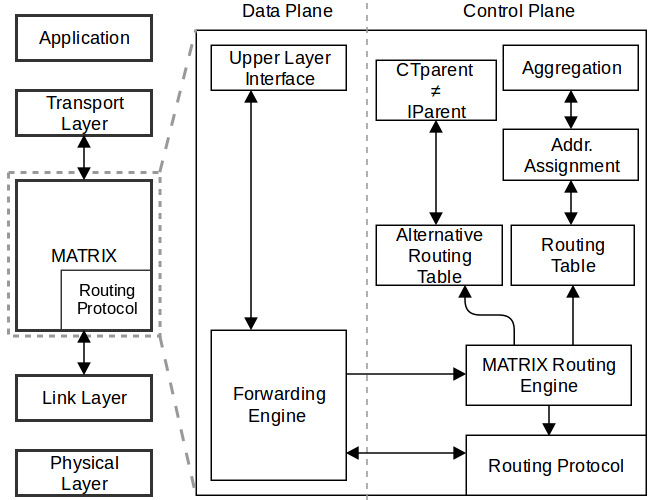
\includegraphics[width=1\columnwidth]{./Images/Architecture.png}
\caption{Matrix protocol's architecture.}
    \label{fig:architecture}
\end{figure}

Matrix is comprised of the following execution phases:
%\begin{enumerate}
 % \item
 
\noindent \textbf{1. Collection tree initialization}: the
  collection tree (Ctree) is built by the underlying collection protocol; each
  node achieves a stable knowledge about who its parent is; adaptive beaconing
  based on Trickle algorithm \cite{Levis:2004} is used to define stability;
  
%  \item
\noindent  \textbf{2. Descendants convergecast,
  IPv6 tree broadcast}: once the collection tree
  is stable, the address hierarchy tree (IPtree) is built using MHCL
  \cite{mhcl}; this phase also uses adaptive beaconing to handle network
  dynamics; by the end of this phase, each node has received an IPv6 address
  range from its parent and each non-leaf node has partitioned its own address 
	space among its children; the resulting address
  hierarchy is stored in the distributed IPtree, which initially has the same
  topology as Ctree, but in reverse, top-down, direction.
  
%  \item
\noindent  \textbf{3. Standard routing}: bottom-up routing is done
  using the collection tree, Ctree, and top-down routing is done using the
  address hierarchy represented by the IPtree; any-to-any routing is performed by combining
  bottom-up forwarding, until the least common ancestor of sender and
  receiver, and then top-down forwarding until the destination.
  
%  \item
\noindent  \textbf{4. Alternative top-down routing table upkeep}: whenever a
node changes its parent in the initial collection tree, it starts sending
  beacons to its new parent in Ctree, requesting to upkeep an entry in
  its routing table with its own IPv6 range; such new links in
  Ctree, in reverse direction, comprise the RCtree routing tables for
  alternative (top-down) routing;
  
%  \item 
\noindent  \textbf{5. Alternative top-down routing via local broadcast}:
whenever a node fails to forward a data packet to the next hop/subtree in the IPtree, it
  broadcasts the packet to its one-hop neighborhood; upon receiving a local
  broadcast, all neighbors check if the destination IPv6 belongs to an address
  range in their RCtree table; if positive, the packet is forwarded to the
  correct subtree of IPtree, otherwise, the packet is dropped; we give a
  geometric argument and show through simulations that such events are rare.
%\end{enumerate}

Next we describe the architecture of Matrix in more detail.

\subsection{IPv6 multihop host configuration}

Matrix is built upon the idea of IPv6 hierarchical address
allocation, proposed in \cite{mhcl, 2016techreport}. Once the collection tree is
stable, the address space available to the border router of the
6LoWPAN, for instance the 64 least-significant bits of the IPv6
address (or a compressed 16-bit representation of the latter), is
hierarchically partitioned among nodes in the collection tree. The
(top-down) address distribution is preceded by a (bottom-up)
convergecast phase, in which each node counts the total number of
its descendants, i.e., the size of the subtree rooted at itself, and
propagates it to its (preferred) parent. Each node saves the number
of descendants of each child. 

Once the root has received the
(aggregate) number of descendants of its $k$ children, it partitions
the available address space into $k$ ranges of size proportional to
the size of the subtree rooted at each child, leaving a portion of
the space as reserve for possible late coming connections (see
Figure~\ref{fig:mhcl}). Each node repeats the address space
partitioning procedure upon receiving its own address range from the
parent and sends the proportional address ranges to the respective
children, until all nodes have received an address. If a new node
connects to the tree after the aggregation phase, it receives an
address range from the reserved space of the respective parent node
(the details of the communication routines used in this phase are
described in detail in \cite{2016techreport}).

Since the address allocation is performed in a hierarchical way, each entry in
the routing table aggregates the addresses of all destination nodes
in the subtree rooted at the corresponding child node. 


%TODO: summarize essencial features of MHCL
\begin{comment}
Once the collection tree Ctree is stable, the IPtree is built using
  MHCL \cite{mhcl}: each node computes the size of its subtree and
  informs its parent in the Ctree; once the root completes the aggregation
  (bottom-up) phase, it partitions the available IPv6 address space (e.g., the least significant 64 bits) among its children, proportionally to
  each subtree's size, and leaves a fixed portion as a reserve for latecomers;
  the address ranges are further partitioned, hierarchically, and sent downwards
  until every node receives an address range (see Figure \ref{fig:mhcl}); if a
  new node connects to the tree after the aggregation phase, it receives an address range from the reserve space of the respective parent node (the
  details of the communication routines used in MHCL are described in detail
  in \cite{mhcl}).
\end{comment}

\begin{figure}[ht]
    \centering
    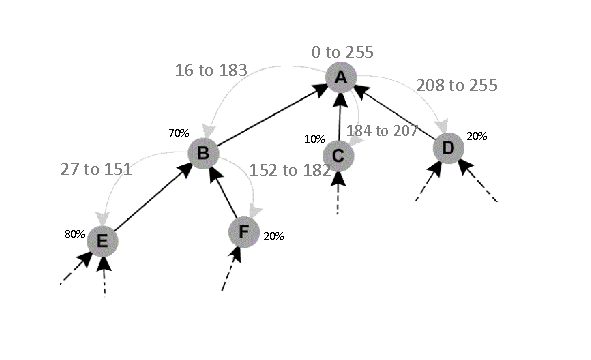
\includegraphics[width=0.9\linewidth]{./Images/mhcl.pdf}
\caption{Example of hierarchical address assignment: (simplified)
scenario with 8-bit available address space at the root and $6.25\%$
of address reserve for delayed connections at each node.}
    \label{fig:mhcl}
\end{figure}

After the address configuration phase, the network initialization is done.
Each node has built the IPtree routing table with the address range of each
child. All table entries are disjoint and sorted in increasing order of
addresses. In this way, message forwarding can be performed in linear time using
one comparison operation per table entry.

%\begin{figure}[ht]
%    \centering
%    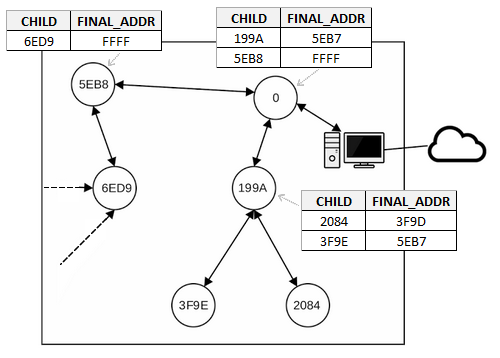
\includegraphics[width=.8\linewidth]{./Images/example.png}
%\caption{Example of routing tables in IPtree.}
%    \label{fig:example}
%\end{figure}


\subsection{Control plane: distributed tree structures}

After the network is initialized and all nodes have received an IPv6
address range, three simultaneous distributed trees are maintained
on all nodes in the 6LoWPAN: \textbf{Ctree:} the collection tree, maintained by the underlying
  collection protocol (CTP/RPL).
  %\item 
	\textbf{IPtree:} the IPv6 address tree, built during the network
  initialization phase and kept static afterwards, except when new
  nodes join the network, in which case they receive an IPv6 range from the reserve space of the respective
parent node in the collection tree.
  %\item 
	\textbf{RCtree:} the reverse collection tree, reflecting the
  dynamics of the collection tree in the reverse direction. Note that in \textit{RCtree},
	each node keeps information about its direct descendents, whereas in \textit{Ctree} each
	node only knows who its parent is.
%\end{itemize}

Initially, IPtree has the same topology as the reverse-collection tree
$Ctree^{R}$, and RCtree has no links (see Figure \ref{fig:t1} and
\ref{fig:t2}).
$$
IPtree = Ctree^{R} \ \text{and} \ RCtree = \emptyset
$$
%, and any-to-any packet forwarding is performed using Ctree for bottom-up and
% IPtree for top-down data flows, respectively.
Whenever a change occurs in one of the links in Ctree, the new link
is added in the reverse direction into RCtree and maintained as long
as this topology change persists (see Figures \ref{fig:t3} and
\ref{fig:t4}).
$$
RCtree = Ctree^{R} \setminus IPtree
$$

Therefore, RCtree is not really a tree since it contains only the
reversed links present in Ctree but not in IPtree. Nevertheless, its
union with the ``working'' links in IPtree is, in fact, a tree,
which is used in the alternative top-down routing:
$$
RCtree \cup (IPtree \cap Ctree^{R}) \  \text{:alternative routing tree.}
$$

\begin{figure}[!h]
\begin{center}
  \subfigure[]
  {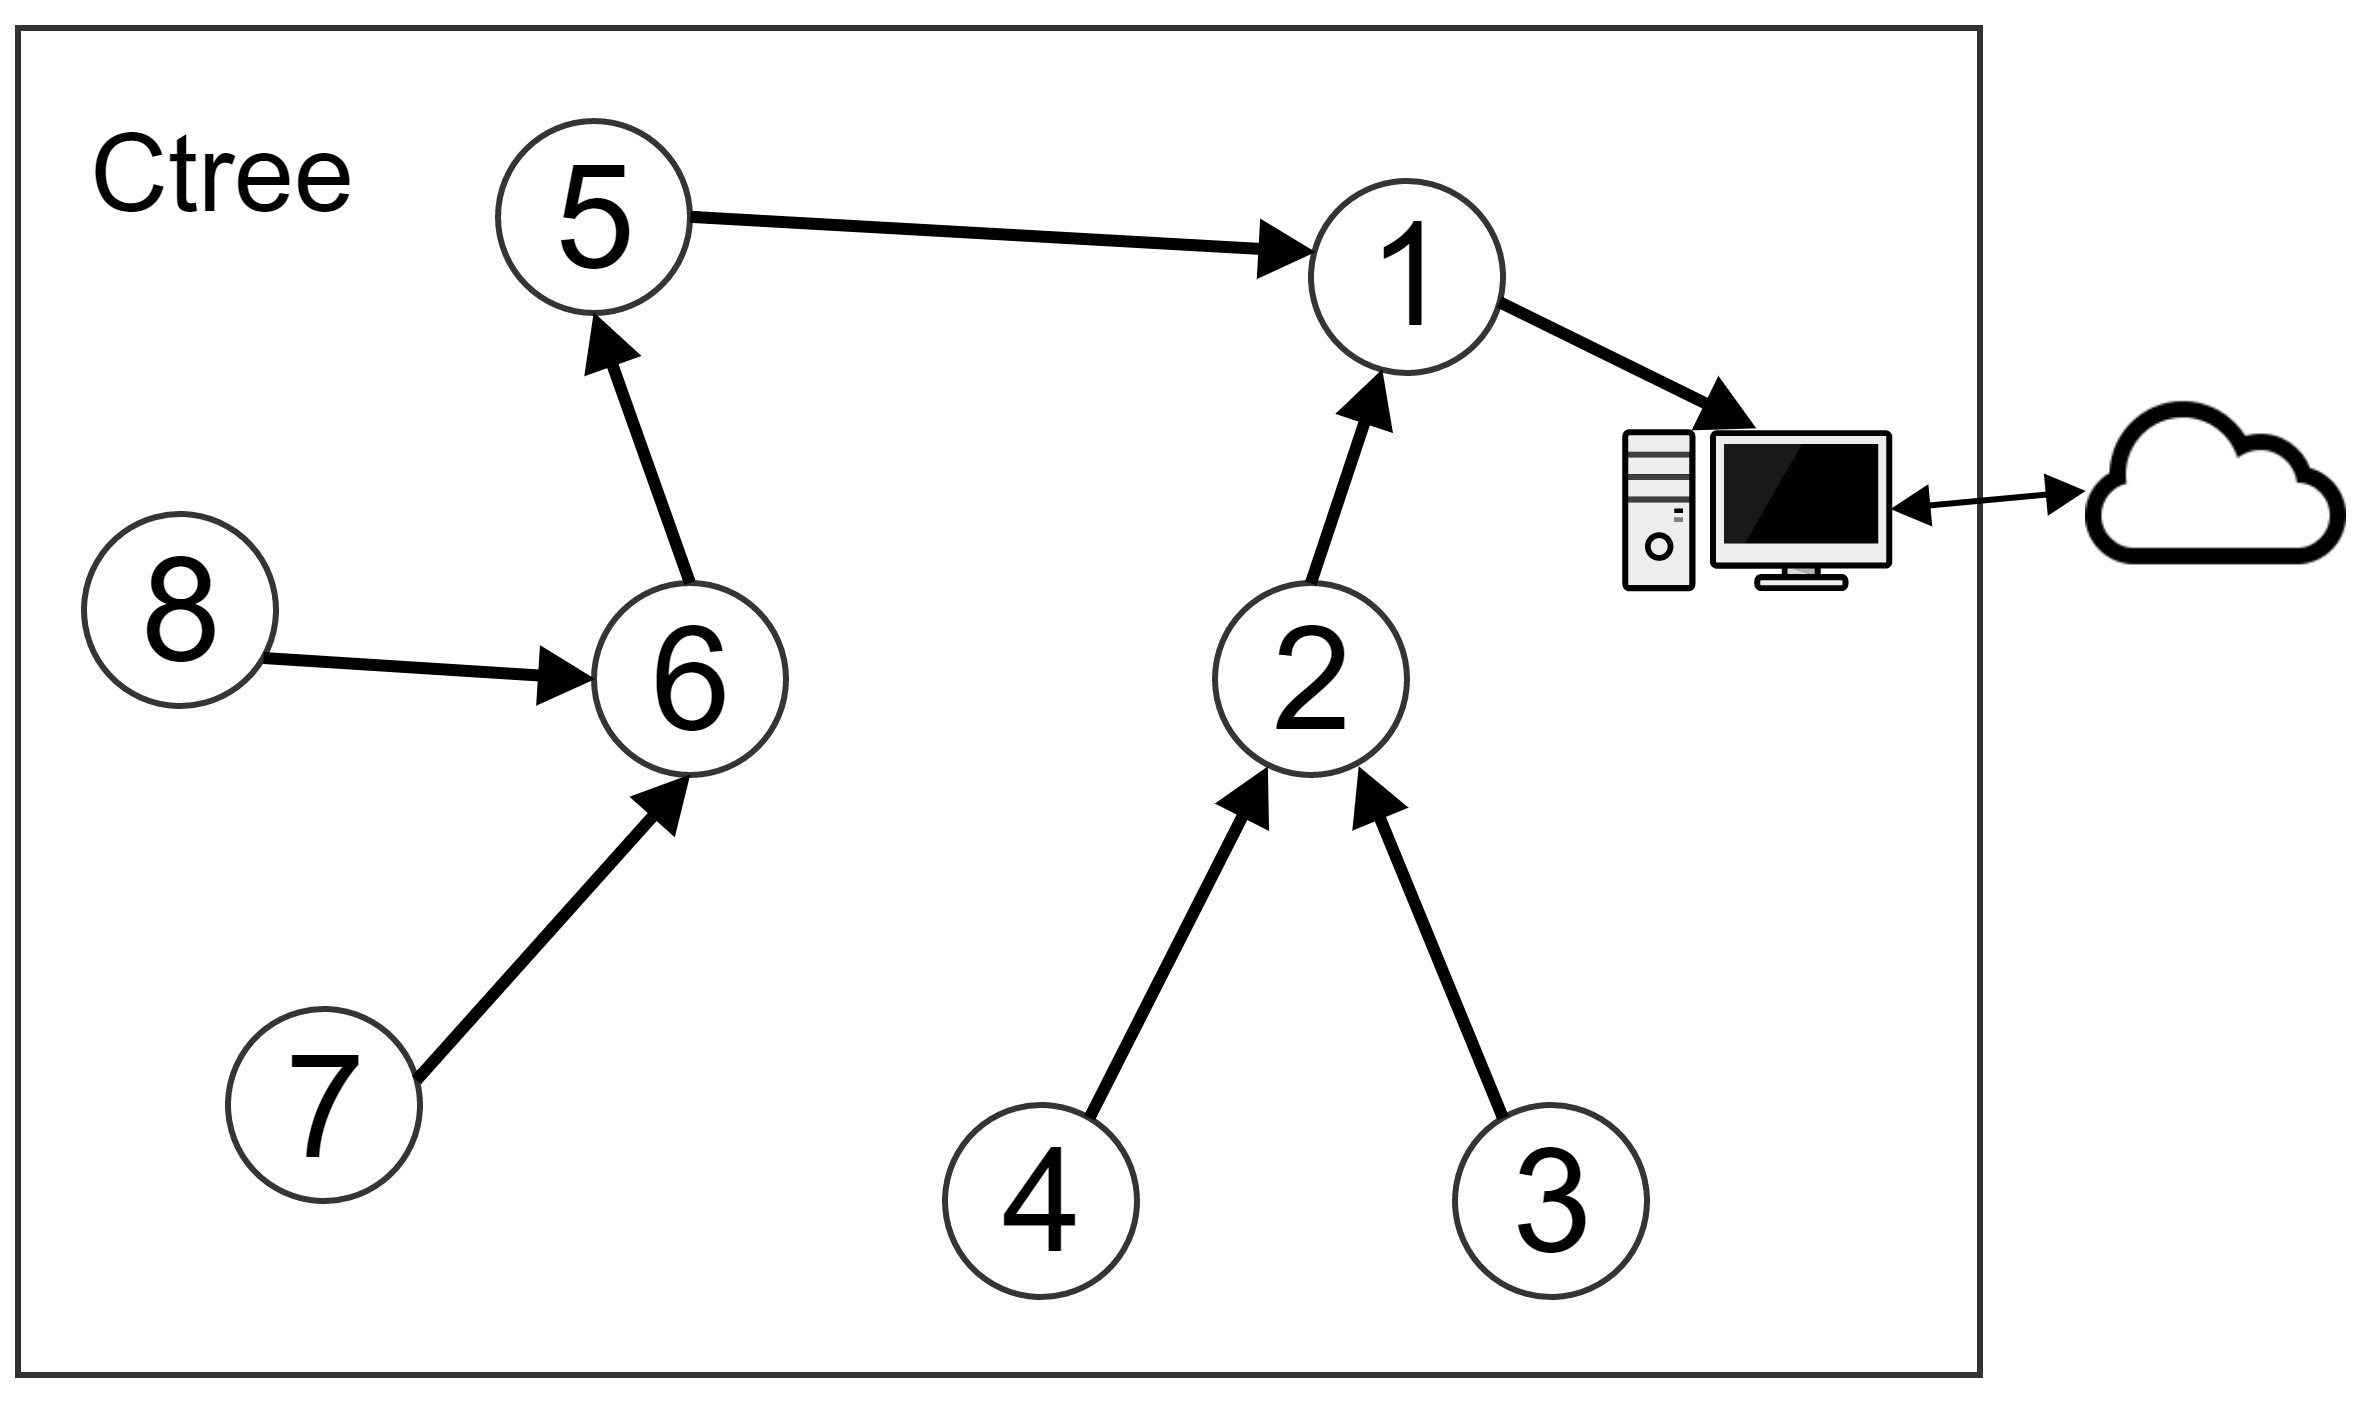
\includegraphics[width=.48\columnwidth]{Images/topologia1.png}
            \label{fig:t1}}
  \subfigure[]
  {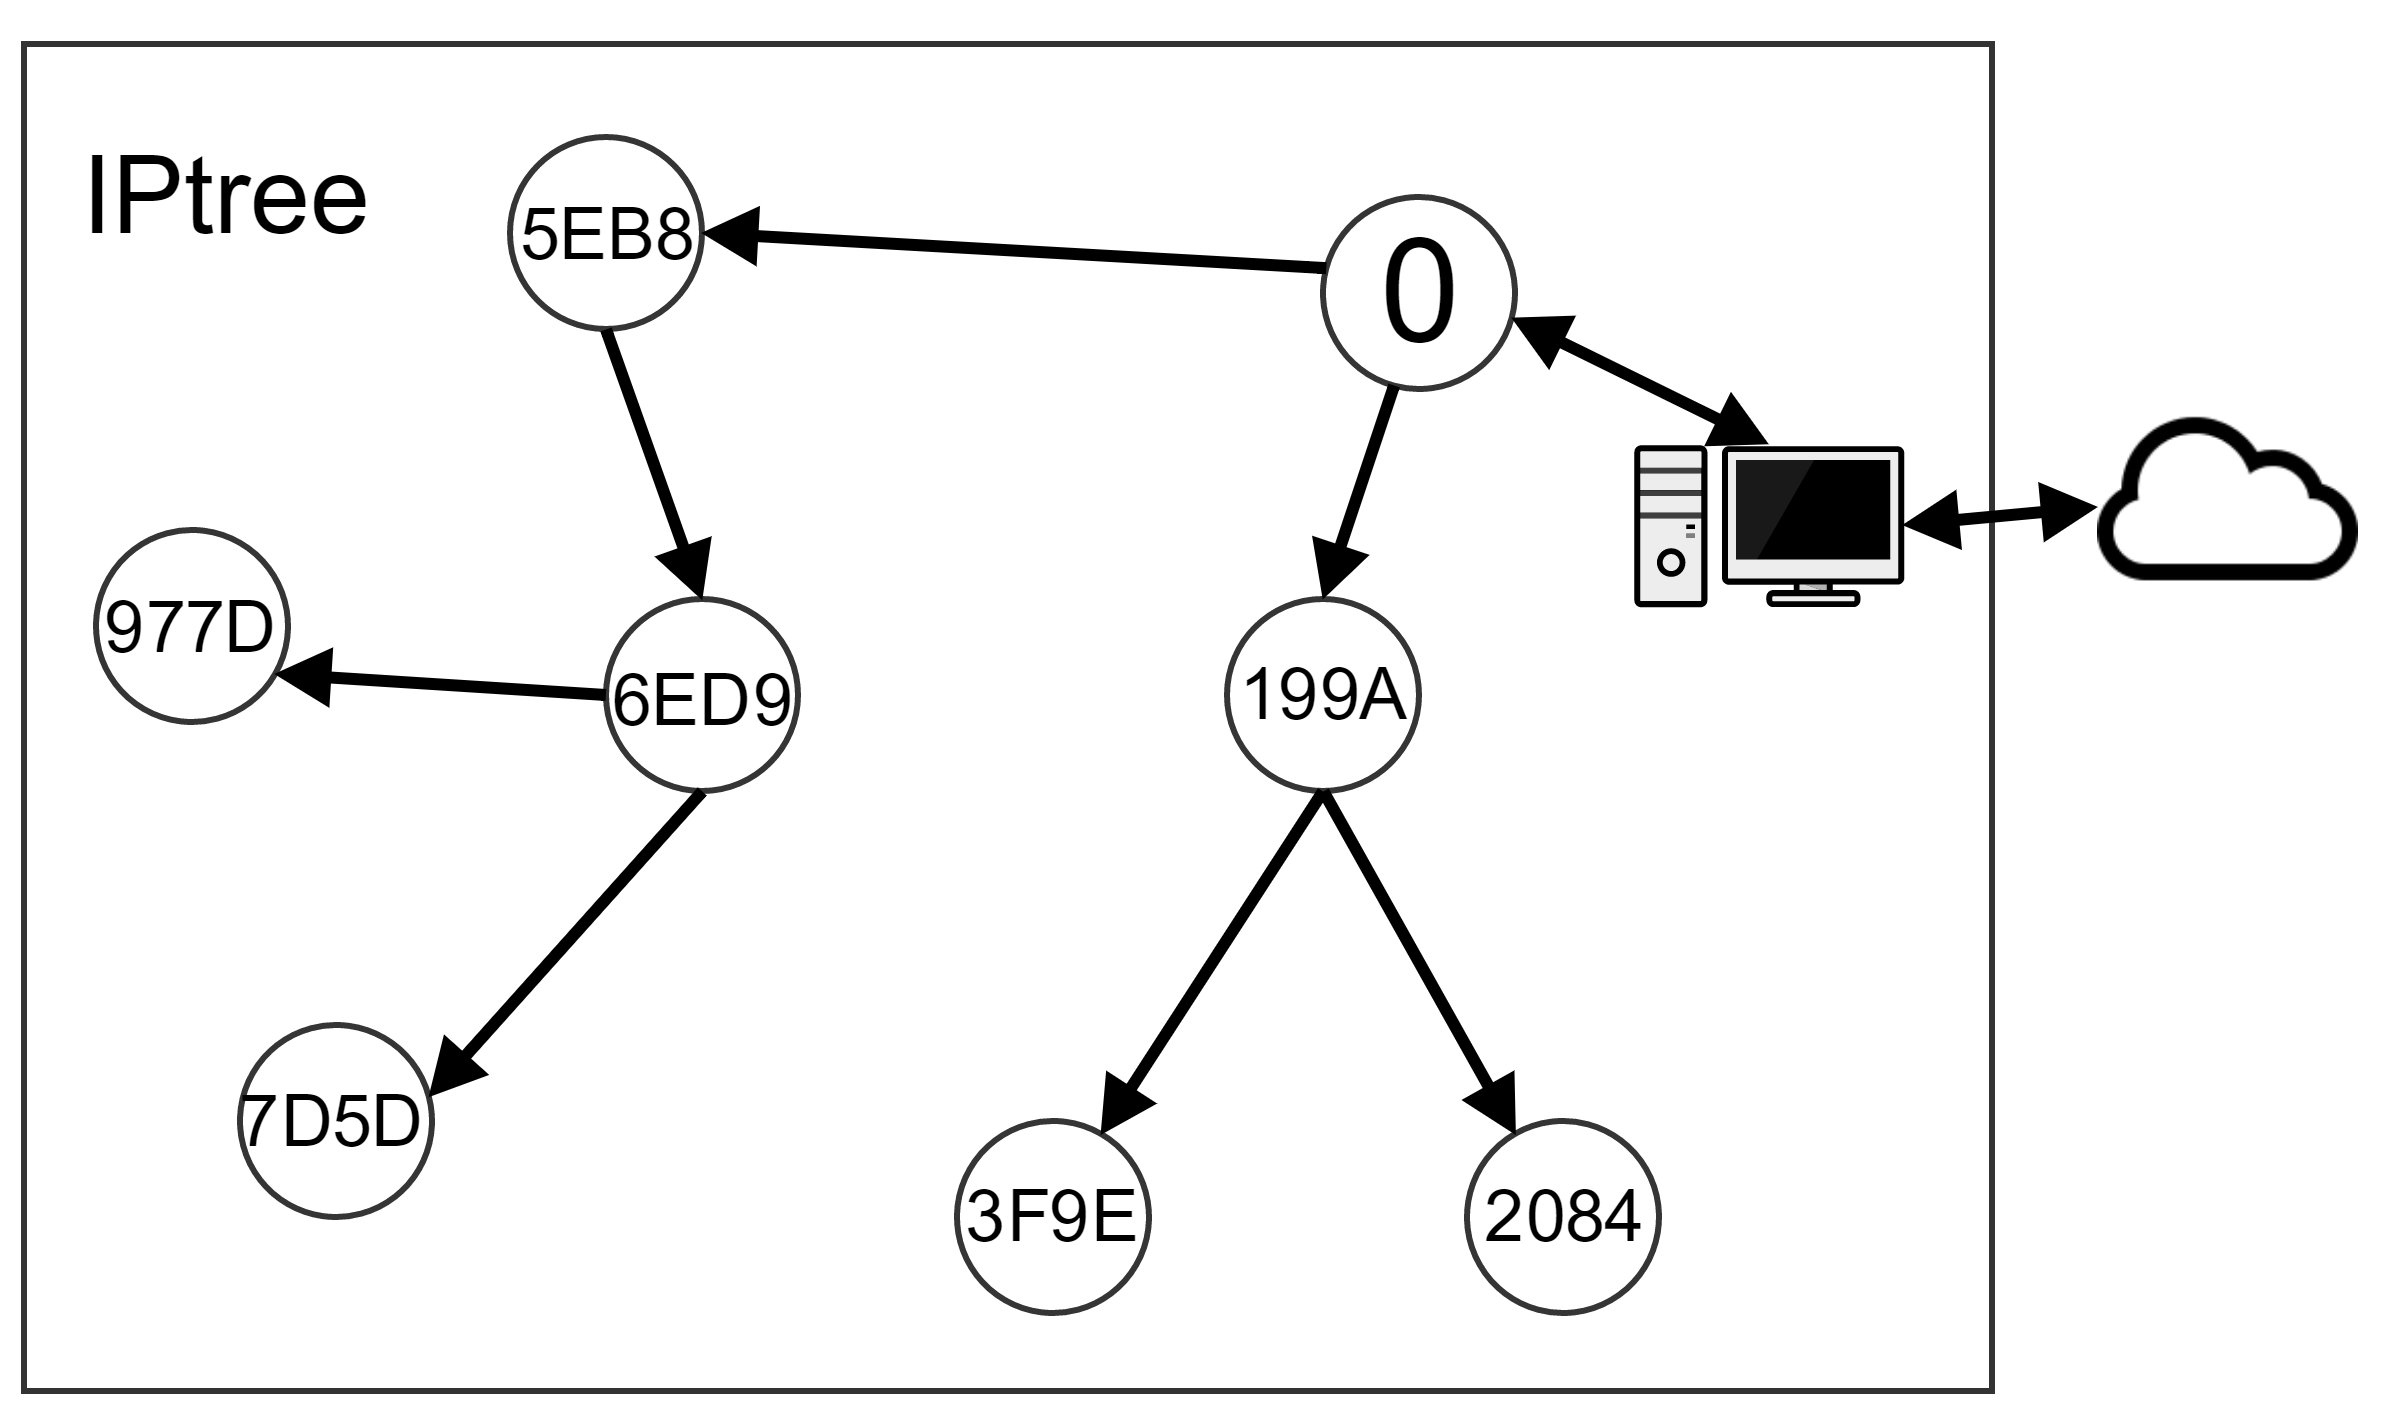
\includegraphics[width=.48\columnwidth]{Images/topologia2.png}
                        \label{fig:t2}}
                            \subfigure[]
  {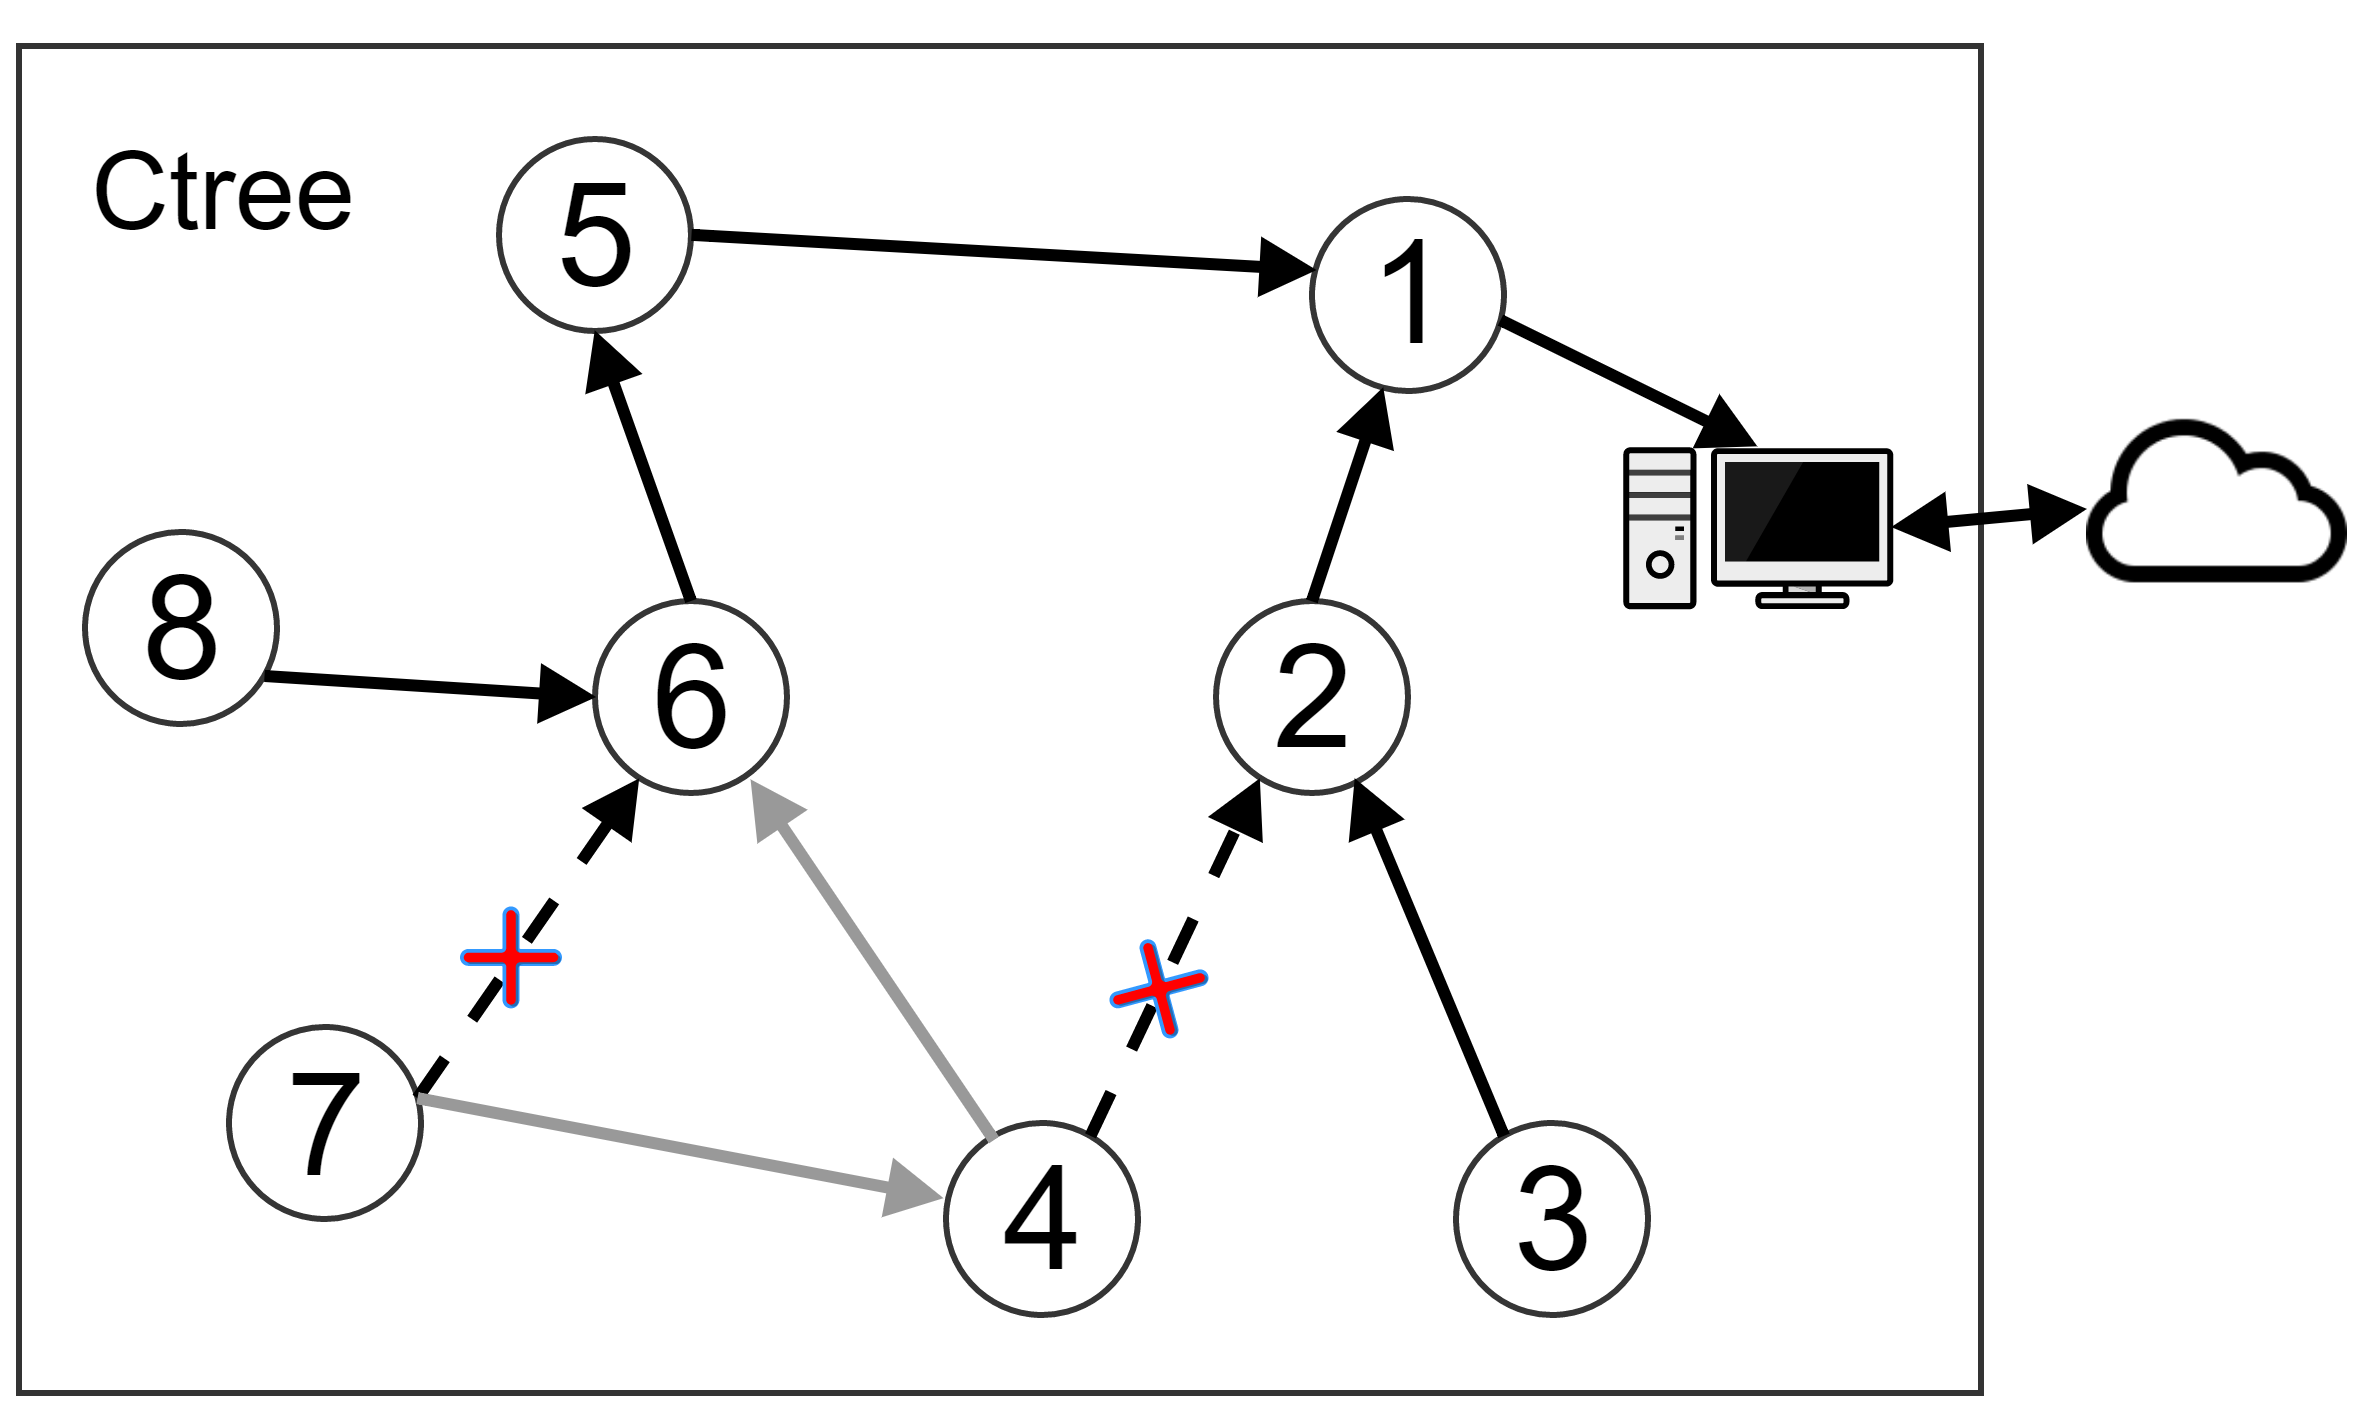
\includegraphics[width=.48\columnwidth]{Images/topologia3.png}
            \label{fig:t3}}
  \subfigure[]
  {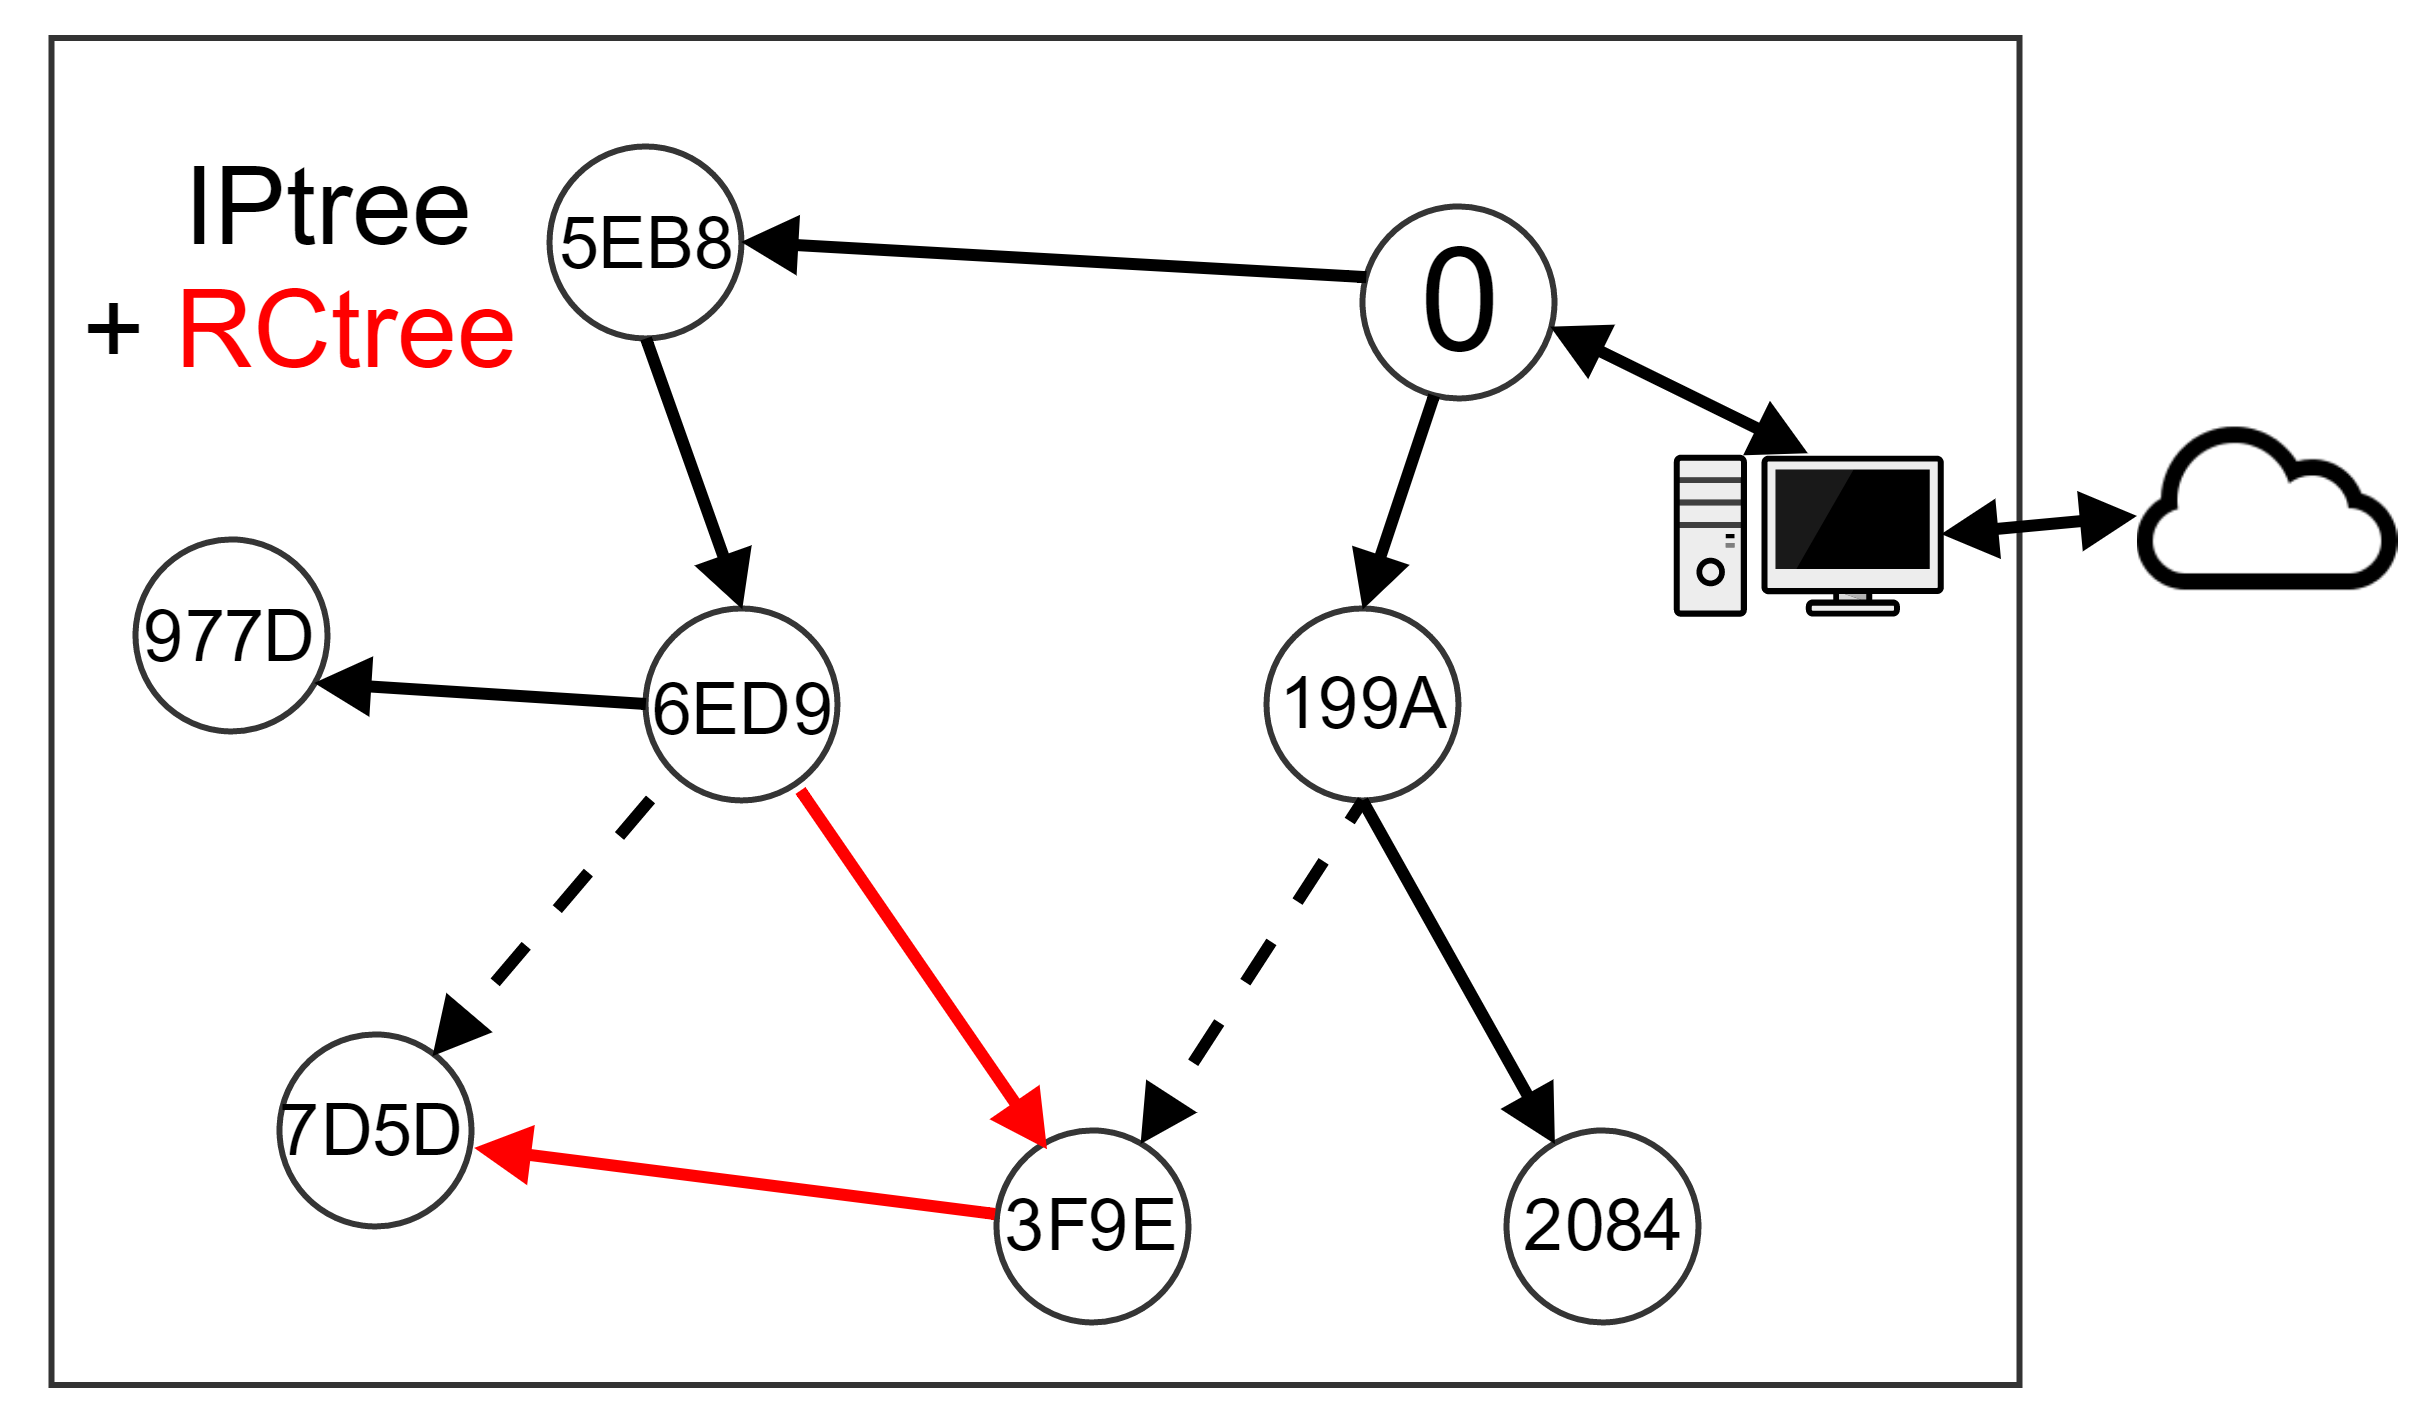
\includegraphics[width=.48\columnwidth]{Images/topologia4.png}
    \label{fig:t4}}
            \caption{RCtree example: before
            and after two links change in the collection tree.}\label{fig:layers}
\end{center}
\end{figure}

Each node $n_i$ maintains the following information:
\begin{itemize}
  \item $CTparent_i$: the ID of the current parent in the dynamic
  collection tree;
  \item $IParent_i$: the ID of the node that assigned $n_i$ its IPv6 range
initially $CTarent_i$ = $IParent_i$);
  \item $IPchildren_i$: the \textit{standard} (top-down) routing table, with
  address ranges of each one-hop descendent of $n_i$ in the IPtree;
  \item $RChildren_i$: the \textit{alternative} (top-down) routing table, with
  address ranges of one-hop descendants in the RCtree.
\end{itemize}

Note that, each node stores only one-hop
neighborhood information, so the memory footprint is $O(k)$, where $k$ is the
number of a node's children at any given moment in time, which is optimal,
considering that any (optimal) top-down routing mechanism would need at
least one routing entry for every (current) child in the tree topology to reach
all destinations.

%TODO: EXPLAIN beacons
The routing engine (see Figure~\ref{fig:architecture}) is responsible for
creating and maintaining the IPtree and RCtree routing tables. IPtree is created
during the network initialization phase, while RCtree is updated dynamically to
reflect changes in the network's link qualities. Whenever a node $n_i$ has its
$CTparent_i$ updated, and the current parent is different from its
$IParent_i$ ($IParent_i \neq CTparent_i$), $n_i$ starts sending periodic beacons
to its new parent, with regular intervals (in our experiments, we set the beacon
interval to $\delta/8$, where $\delta$ is the maximum interval of the
Trickle timer used in CTP).
Upon receiving a beacon (from a new child in the collection tree), a node
($n_j = CTparent_i$) creates and keeps an entry in its alternative
routing table $RChildren_j$ with the IPv6 address range of the subtree of $n_i$. As soon as $n_i$
stops using $n_j$ as the preferred parent, it stops sending beacons to $n_j$.
If no beacon is received from $n_i$ after $2\times\delta$ ms, its (alternative)
routing entry is deleted. Therefore, links in RCtree are temporary and are deleted when not present in neither the
collection nor the IP trees.

\begin{comment}
Figure \ref{fig:layers} shows an overview of network and transport layers, using
MATRIX in between. CTP performs the construction of a routing tree, where each
node is represented by a fixed identifier. MATRIX allows communication in both
directions and uses IPv6, enabling direct communication with the Internet. The
transport layer can perform end-to-end communication between two nodes using
IPv6. TODO: EXPLAIN DIFFERENT TREES
\end{comment}

%\begin{figure}[!ht]
%    \centering
%    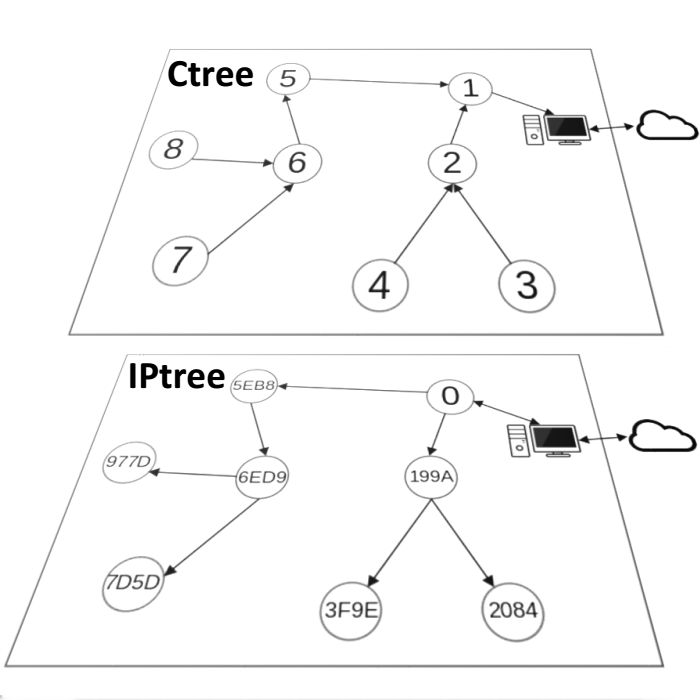
\includegraphics[width=1\linewidth]{./Images/layers2.png}
%\caption{Protocol layers using MATRIX TODO: SHOW DIFFERENT TREES}
%    \label{fig:layers}
%\end{figure}




\subsection{Data plane: any-to-any routing}


The forwarding engine (see Figure~\ref{fig:architecture}) is responsible for
application packet forwarding. Any-to-any routing is performed by combining
  bottom-up forwarding, until the least common ancestor of sender and
  receiver, and then top-down forwarding until the destination. Upon receiving
  an application layer packet, each node $n_i$ verifies whether the destination IPv6 address falls within some range
$j \in IPchildren_i$: if yes then the packet is forwarded
(downwards) to node $n_j$, otherwise, the packet is forwarded
(upwards) to $CTparent_i$. Note that, since each node has an IPv6
address, in contrast to collection protocols, such as CTP and RPL,
in Matrix, every node can act as a destination of messages
originated inside and outside of the 6LoWPAN.

Each forwarded packet requests an acknowledgment from the next hop and can be
retransmitted up to 30 times (similarly to what is done in CTP
\cite{Fonseca:2009}). If thereafter no acknowledgment
is received, then the node performs a \textit{local broadcast}, looking for an
alternative next hop in the RCtree table of a (one-hop) neighbor. The
\textit{alternative routing} process is described in detail below.


\subsection{Fault tolerance and network dynamics}


So why is Matrix robust to network dynamics? Note that, since
routing is based on the hierarchical address allocation, if a node
with the routing entries necessary to locate the next subtree
becomes unreachable for longer than approximately one second
(failures that last less than 1s are effectively dealt with by
retransmission mechanisms available in standard link layer
protocols), messages with destinations in that subtree are dropped.

When a node or link fails or changes in Ctree, RCtree reflects this
change, and packets are forwarded from IPtree to RCtree via a local
broadcast. The node that receives a local-broadcast checks in its
RCtree whether it knows the subtree of the destination IPv6 address:
if yes then is forwards the packet to the right subtree and the
packet continues its path in the IPtree until the final destination.

\begin{figure}[!h]
\begin{center}
  \subfigure[]
  {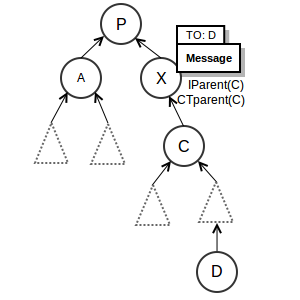
\includegraphics[width=.48\columnwidth]{Images/lb1.png}
            \label{fig:lb1}}
  \subfigure[]
  {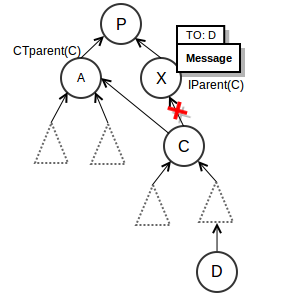
\includegraphics[width=.48\columnwidth]{Images/lb2.png}
                        \label{fig:lb2}}
                            \subfigure[]
  {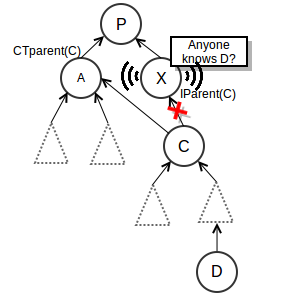
\includegraphics[width=.48\columnwidth]{Images/lb3.png}
            \label{fig:lb3}}
  \subfigure[]
  {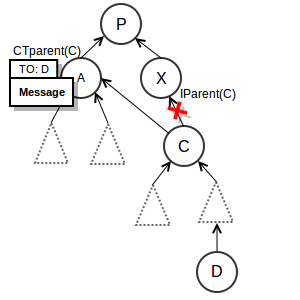
\includegraphics[width=.48\columnwidth]{Images/lb4.png}
    \label{fig:lb4}}
            \caption{Alternative top-down routing.}\label{fig:localbroadcast}
\end{center}
\end{figure}


Consider the following scenario: node X receives a packet with destination IPv6
address D (see Figure \ref{fig:lb1}). After consulting its standard routing
table $IP-children_X$, X forwards the packet to C. However, the link X
$\Rightarrow$ C fails, for some reason, and C does not reply with an
acknowledgment.
Then, X makes a constant number (e.g., 30 times in CTP) of retransmission
attempts. Meanwhile, since node C also lost its connection to X, it decides to
change its parent in the collection tree to node A (see Figure \ref{fig:lb2}).
Having changed its parent, C starts sending beacons to A, which creates an entry
in its alternative routing table $RC-children_A$ for the subtree rooted at C, and
keeps it as long as it receives periodic beacons from C (which will be done as long as $CTparent_C$ = A).

Having received no ack from C, X activates the \textit{local
broadcast} mode: it sets the message's type to ``LB'' and broadcasts
it to all its one-hop neighbors (see Figure \ref{fig:lb3}). Upon
receiving the local broadcast, node A consults its alternative
routing table and finds out that the destination address D falls
within the IPv6 address range C. It then forwards the packet to C,
from where the packets follows along its standard route in the
subtree of C (see Figure \ref{fig:lb4}).

Note that this
mechanism does not guarantee that the message will be delivered. If no one-hop
neighbor of X had the address range of C in its alternative routing table, then
the packet would be lost. Nevertheless, we argue that the probability that the
message will be forwarded to the appropriate subtree is high.

\subsection{Alternative routing: geometric rationale}

%TODO: introduce the problem, why local broadcast does not guarantee delivery
%even when there is a path
The success of the local broadcast mechanism lies in the ability to forward
messages top down along the IPtree, in spite of one or more link or node
failures on the way.
%Note that, whenever a node of IPtree is unavailable, it
%might not be possible to find the right subtree of the destination.
Matrix is designed to handle (non-adjacent) link or node failures and relies on
a single local broadcast and temporary reverse collection links (RCtree).

Consider once again the scenario illustrated in Figure \ref{fig:localbroadcast}.
When a node X is unable to forward a packet to the next hop, it activates the
local broadcast mechanism, and it becomes essential that one of X's one-hop
neighbors (in this case A) has replaced X as a parent of C in
the collection tree. Therefore, given that the new parent of C is A, it becomes
essential that X and A are neighbors. We argue that it is unlikely that this is not the case.

\begin{figure}[!ht]
    \centering
    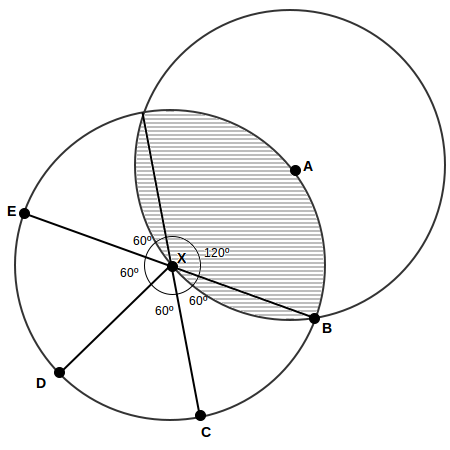
\includegraphics[width=.6\linewidth]{./Images/localBroadcast.png}
\caption{UDG model: the number of independent neighbors of X is at most 5.}
    \label{fig:udgIndN}
\end{figure}

Our argument is of geometric nature. Since the considered 6LoWPAN is
wireless, we show our argument in a unit disk graph (UDG) model
\cite{Clark:1991}. We use the fact that the number of independent neighbors of
any node in a UDG is bounded by a small constant, namely 5. The proof of this
fact is sketched in Figure \ref{fig:udgIndN}: consider a node X and its neighbor
A. Any node located inside the gray region is a neighbor of both X and A, so any
neighbor of X that is independent of (not adjacent to) A has to be outside the
gray area and inside the circle around X. Let's call this neighbor B. The next
independent neighbor of X has to be located outside the 60 degree sector that
starts at B, and so on. This procedure can be repeated no more than 5 times,
before the 360 degrees around X are covered.

Given that the maximum number of neighbors that do not know each
other is very small, for any possible node distribution and density
around X, the probability that two neighbors of X are independent is
low. In Figure \ref{fig:lb3}, since both X and A are neighbors of C,
the probability that they are themselves neighbors is high. Similar
arguments can be used to back the effectiveness of the local
broadcast mechanism when dealing with different non-adjacent link
and node failures.

Note that this reasoning is only valid in an open space without obstacles and,
even then, does not guarantee that the message will be delivered. Nevertheless,
our experiments show that this intuition is in fact correct, and Matrix has a
95\%--99\% message delivery success in scenarios with node failures of
increasing frequency and duration.

%\subsection{IPv6 hierarchical address allocation}\label{sec:mhcl}

MHCL partitions the address space available to the border router, for instance the 64 least-significant bits of the IPv6 address (or a compressed 16-bit representation of the latter), hierarchically among nodes connected to the border router through a multihop cycle-free topology (implemented by standard protocols, such as RPL~\cite{rfc6550} or CTP~\cite{Fonseca:2009}). Each node
receives an address range from its parent and partitions it among its children, until all nodes receive an address (see Figure \ref{fig:mhcl}). Since the address allocation is performed in a hierarchical way, the routing table of each node can have $k$ entries, where $k$ is the number of its (direct) children. Each routing table entry aggregates the addresses of all nodes in the subtree rooted at the corresponding child-node. However, MHCL does not handle tree topology dynamics, i. e., a failure on a node or link can cause some local topology changes, which can break the hierarchical nature of MHCL. In \cite{mhcl}, only packet loss were handled. Therefore, it is necessary to design a mechanism to cope with local topology changes able to maintain routing with low memory footprint.

\begin{figure}[!ht]
    \centering
    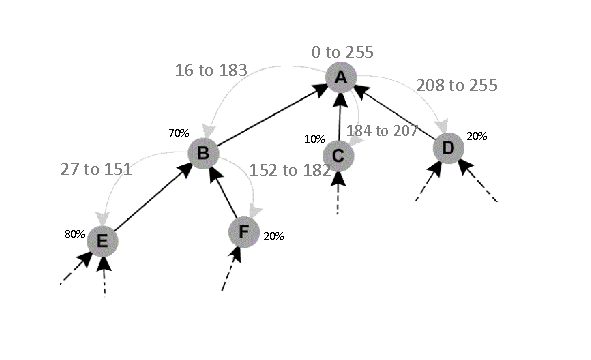
\includegraphics[width=1\linewidth]{./Images/mhcl.pdf}
\caption{Example of MHCL address assignment. 8-bit address space at the root and $6.25\%$ of address range reserved for future/delayed connections}
    \label{fig:mhcl}
\end{figure}

In order to decide how the available address space is partitioned, nodes need to collect information about the topology of the network. To do this, each node $n_i$ counts the total number of its descendants, i.e., the size of the subtree rooted at itself, and propagates it to its parent. Moreover, $n_i$ saves the number of descendants of each child. Once the root has received the number of descendants of each child, it partitions the available address space into $k$ slices of size proportional to the size of the subtree rooted at each child, also leaving a portion of $r\%$ as reserve. Each node $n_i$ repeats the space partitioning procedure upon receiving its own address space from the parent and sends the proportional address slices to the respective children. The idea is to allocate larger address portions to larger subtrees, which becomes important in especially large networks, because it maximizes the address space utilization. Experiments in \cite{mhcl} shown that MHCL is efficient in number of messages and time. Nevertheless, due to simulations' constraints, the results were not satisfactory and only few scenarios were evaluated. In addition, there were a lot of dependency between the proposed protocol and RPL, which can affect the results.


\begin{comment}
MATRIX is a platform-independent routing scheme that extends an underlying
(collection) tree topology (provided by CTP or RPL) and enables any-to-any data
flows in a scalable and dynamic fashion.
MATRIX maintains two coexisting trees: one for the hierarchical IPv6 addressing
($IPtree$), which is built based on the first stable tree topology; and the
second tree for dynamic reverse collection ($RCtree$), reflecting the dynamics
of the collection tree (or DAG). MATRIX enable efficient and robust any-to-any
IPv6 routing with low memory footprint. This is done by implementing an IPv6
address allocation scheme, first proposed in \cite{mhcl}. The low memory
footprint is achieved due to the small routing table entries: each node stores
$k$ entries, where $k$ is the number of its direct children.

Matrix adapts to the network dynamics, since it constructs an
alternative downward routing table to store alternative local routes in case of node and
link failures. This mechanism is proactive and keeps track of local topology
changes or link and node failures. It is also scalable because, taking advantage
of the hierarchical addressing, it does not need to store individual IPv6
address of the downward destination. By only storing the IPv6 address range of a
certain node, MATRIX can perform alternative routing to the subtree rooted at
this certain node.

Every time a local topology change occurs, originated from a node or link
failure, the hierarchical nature of MHCL may be lost. However, we don't want to
compromise the routing by given a node another IPv6 address compatible with its
new hierarchy. This would trigger the addressing of a whole subtree every time a
failure occurs. Instead of doing this, a node keep track of who its $IP-parent$
is, i. e., the node that gave him its address. When the node's parent it's no
longer its $IP-parent$, the node must send beacons to inform the new parent
about its existence. We will call the new parent $RC-parent$ (the parent on the
$RCTree$) and, consequently, the node is an $RC-child$. When the node notices
that its $current-parent$ changed, and the new parent isn't the $IP-parent$, it
triggers an event responsible for sending beacons to the $RC-parent$. This
beacons are sent in a fixed interval, called $\delta$, in order to make the
$RC-parent$ keep an entry in the $RC routing table$ for the  $RC-child$. The
$RC-parent$ should store the IP range from its $RC-children$ in the $RC routing
table$. This $RC routing table$ will store only $RC-children$ and each entry
have a validity field, responsible for erasing the entry if no beacons is received after $2\times\delta$.

Figure \ref{fig:localbroadcast} shows an example of a topology change due to
link failure and how MATRIX route the message using alternative routes. When a
message arrives at a node $X$ to be routed to a destination $D$, $X$ must look
into its table and decide if this message should be forwarded to one of its
$IP-children$ $C$, if the destination address is contained in the address range
from $C$, or to its parent $P$, otherwise (Figure \ref{fig:lb1}). If this
message is forwarded to $C$, the node $X$ waits for an acknowledgment. Based on
CTP implementation, $X$ can perform 30 retransmissions. After all these
attempts, if an acknowledgment has not been received, probably $C$ is no longer
a child of $X$ (Figure \ref{fig:lb2}). Node $X$ will then trigger a local
broadcast searching for $D$. All one hop neighbors from $X$ will receive this
broadcast message and must look into theirs $RC routing table$s to find out if
$D$ is now its $RC-descendent$, i. e., $D$ is a descendant from an $RC-child$
(Figure \ref{fig:lb3}). Upon receiving a response from one of his neighbors, in
this case $A$, about the knowledge of the destination $D$, $X$ then forward the message to $A$ that consequently routes the message to $D$ (Figure \ref{fig:lb4}).


\subsection{MATRIX protocol states}\label{subsec:states}
 When running MATRIX protocol, a node can be in one of seven different computing states. Each of the states and what they represent are described below.
\begin{itemize}
    \item $S_{0}$ Tree not stable: During this step, the tree is being built by a routing protocol, according to some metric. A node have not yet decided who its parent is. To decide if a node is $stable$, MATRIX implements a Trickle-based timer, so CTP can construct the routing tree before the aggregation starts.
    \item $S_{1}$ Descendants aggregation: As soon as the network is considered $stable$, MATRIX initializes the aggregation routine. Every node, except the root, starts sending aggregation messages to its parent, with its descendants number. For each new message received from a child $c_i$, the node updates the descendants information of $c_i$ and, after the aggregation timer is complete, sends an updated message to its parent. Every time a new message arrives, a Trickle-based timer is reset. This is done to be energy aware, reducing the number of transmissions.
    \item $S_{2}$ Aggregation done: When this second Trickle-based timer hits its limit, if the node is the root, it considers that the aggregation phase is finished and starts addressing.
    \item $S_{3}$ IP distribution: When in this state, a node must take its address slice (received from its $IP-parent$) and divide it, proportionally, among its children, given the number of descendants computed on the aggregation phase. A node must also save a reserve address range, for latecomers children.
    \item $S_{4}$ Addressing done: After addressing its children, a node considers the addressing step finished.
    \item $S_{5}$ Latecomer nodes: After the addressing done, if the node receives
    a request for address from a child, it considers that child a latecomer and gives a slice of its reserve address range for it.
    \item $S_{6}$ $Current-parent$ $=$ $IP-parent$: While in this state, the protocol is working on its standard routing.
    \item $S_{7}$ $Current-parent$ $\neq$ $IP-parent$: If a node changes its
    parent, the address hierarchy is broken. In order to maintain the routing
    without the need to assign a new address, the node must send beacons in a
    fixed interval to its $RC-parent$, so this $RC-parent$ can store its address range in an $RC routing table$.
\end{itemize}
\end{comment}

\section{Complexity Analysis}\label{sec:analysis}

In this section, we assume a synchronous communication model with
point-to-point message passing. In this model, all nodes start
executing the algorithm simultaneously and time is divided into
synchronous rounds, i.e., when a message is sent from node $v$ to
its neighbor $u$ at time-slot $t$, it must arrive at $u$ before
time-slot $t+1$.

We first analyze the message and time complexity of the IPv6 address
allocation phase of Matrix. Then, we look into the message
complexity of the control plane of Matrix after the network
initialization phase.

Note that Matrix requires that an underlying acyclic topology (Ctree) has
been constructed by the network before the address allocation starts, i.e.,
every node knows who its parent in the Ctree is.
Moreover, one of the building blocks of Matrix is the address allocation phase, described in Section~\ref{subsec:mhcl}.

\begin{theorem} For any network of size $n$ with a
spanning collection tree $Ctree$ rooted at node $root$, the message and time
complexity of Matrix protocol in the address allocation phase is
Msg$(Matrix^{IP}$ $(Ctree, root))$ = $O(n)$ and Time $(Matrix^{IP}$ $(T, root))$
= $O(depth(Ctree))$, respectively. This message and time complexity is
asymptotically optimal.
\end{theorem}
\begin{proof}
The address allocation phase is comprised of a tree broadcast and a tree
convergecast.
In the broadcast operation, a message (with address allocation information) must be
sent to every node by the respective parent, which needs $\Omega(n)$ messages.
Moreover the message sent by the root must reach every node at distance
$depth(Ctree)$ hops away, which needs $\Omega(depth(Ctree))$ time-slots.
Similarly, in the convergecast operation, every node must send a message to its
parent after having received a message from its children, which needs
$\Omega(n)$ messages. Also, a message sent by every leaf node must reach the
root, at distance $\leq depth(Ctree)$, which needs $\Omega(depth(Ctree))$
time-slots.
\end{proof}

Next, we examine the communication cost of the routines involved in
the alternative routing, performed in the presence of persistent
node and link failures.

\begin{theorem} Consider a network with $n$ nodes and a failure event that
causes $\mathcal{L_{CT}}$ links to change in the collection tree Ctree for at
most $\Delta$ ms.
Moreover, consider a beacon interval of $\delta$ ms.
The control message complexity of Matrix to perform
alternative routing is $Msg(Matrix^{RC})$ = $O(n)$.
\end{theorem}
\begin{proof}
Consider the $\mathcal{L_{CT}}$ link changes in the collection tree
Ctree. Note that $\mathcal{L_{CT}} = O(n)$ since Ctree is acyclic
and, therefore, has at most $n-1$ links. Every link that was changed
must be inserted in the RCtree table of the respective (new) parent
and kept during the interval $\Delta$ using regularly sent beacons
from the child to the parent. Given a beacon interval of $\delta$,
the total number of control messages is bounded by
${\Delta}/{\delta} \times \mathcal{L_{CT}} = O(n)$.\end{proof}

Note that, in reality, the assumptions of synchrony and
point-to-point message delivery do not hold in a 6LoWPAN. The moment
in which each node joins the tree varies from node to node, such
that nodes closer to the root tend to start executing the address
allocation protocol earlier than nodes farther away from the root.
Moreover, collisions, node and link failures can cause delays and
prevent messages from being delivered. We analyze the performance of
Matrix in an asynchronous model with collisions and transient node
and link failures of variable duration through simulations in
Section~\ref{sec:results}.

\section{Evaluation}
\label{sec:results}

In this section, we evaluate the performance of Matrix through
simulations.

\subsection{Simulation setup}\label{subsec:sim}

Matrix was implemented as a subroutine of CTP in TinyOS \cite{tinyos}
and the experiments were run using the TOSSIM simulator~\cite{tossim}. We
compare Matrix with and without the local broadcast mechanism, to which we refer
as MHCL (note that the implementation is
different from that in \cite{2016techreport}, where it was implemented as a
subroutine of RPL). RPL was implemented in Contiki \cite{Dunkels:2004} and was
simulated on Cooja~\cite{Eriksson:2009}. Table \ref{tab:conf} lists the default
simulation parameters used for each protocol, in a non-faulty scenario. We use the $LinkLayerModel$ tool from TinyOS to generate the topology and connectivity model. 
We simulated a range of faulty scenarios, based on experimental data collected
from TelosB sensor motes, deployed in an outdoor
environment \cite{Baccour:2012}. In each scenario, after every 60 seconds of
simulation, each node shutdowns its radio with probability $\sigma$ and keeps
the radio off for a time interval uniformly distributed in
$[\varepsilon - 5, \varepsilon + 5]$ seconds (see Table~\ref{tab:scn}).
The first scenario ($Scn1$) represents a network without node failures. The
remaining scenarios represent a combination of values of $\sigma$ and
$\varepsilon$. Note that these are all node-failure scenarios, which are
significantly harsher than models that simulate link or per-packet
failures only.

On top of the network layer, we ran an application, in which each node
sends 10 messages to the root, and the root relies with an ack. Nodes start sending application messages 90 seconds after the simulation has started. The entire
simulation takes 20 minutes. Each simulation was run 10 times. In each plot,
the curve or bars represent the average, and the error bars the confidence
interval of 95\%.

\begin{table}[!ht]
\centering
\caption{Simulation parameters}
\label{tab:conf}
\begin{tabular}{@{}lc@{}}
\toprule
\multicolumn{1}{l}{\textbf{Parameter}} & \textbf{Value} \\ \midrule
Base Station                           & 1 center       \\
Number of Nodes                        & 100            \\
Radio Range ($m$)                      & 100            \\
Density ($nodes/m^{2}$)                & 10             \\
Number of experiments                              & 10             \\
Path Loss Exponent                     & 4.7            \\
Power decay (dB)                       & 55.4           \\
Shadowing Std Dev (dB)                 & 3.2            \\
Simulation duration                 & 20 min            \\
Application messages (node to root + ack)  & 10 per node \\
Max. Routing table size & 20 entries \\
\bottomrule
\end{tabular}
\end{table}

\begin{table}[]
\centering
\caption{Faulty network scenarios}
\label{tab:scn}
\begin{tabular}{|c|c|c|c|}
\hline
\textbf{$\sigma$$\setminus$$\varepsilon$} & \textbf{10 sec.} & \textbf{20 sec.} & \textbf{40 sec.}\\ \hline
\textbf{1\%}     & Scenario 2            & Scenario 3        & Scenario 4              \\ \hline
\textbf{5\%}     & Scenario 5            & Scenario 6        & Scenario 7             \\ \hline
\textbf{10\%}    & Scenario 8            & Scenario 9        & Scenario 10              \\ \hline
\end{tabular}
\end{table}


\subsection{Results}\label{subsec:res}

Firstly, we turn our attention to memory efficiency of each protocol.
To evaluate the usage of routing tables, we compare the number of entries used
by each protocol. Each node was allocated a routing table of equal maximum size:
20 entries.
In Figure \ref{fig:table-usage}, we show the CDFs (cumulative distribution
functions) of the percentage of routing table usage among nodes\footnote{We
measured the routing table usage of each node in one-minute intervals, then
took the average over 20 minutes. }), and compare Matrix,
RPL, and MHCL.
In this plot, Matrix was simulated in the faulty scenario \#10 (Table \ref{tab:scn}).
Note that $>35\%$ of nodes are leaves,
i.e., do not have any descendants in the collection tree topology,
and therefore use zero routing table entries.
As we can see, RPL is the only protocol that uses 100\% of table
entries for some nodes ($\geq30\%$ of nodes have their tables full).
This is due to the fact that RPL, in the storing mode, pro-actively
maintains an entry in the routing table of every node on the path
from the root to each destination, which quickly fills the available
memory and forces packets to be dropped. 
The difference between MHCL and Matrix is small: MHCL
stores only the IPtree structure, whereas Matrix stores IPtree and
RCtree data; the latter is kept only temporarily during parent
changes in the collection tree, so its average memory usage is low.

\begin{figure}[h]
    \centering
    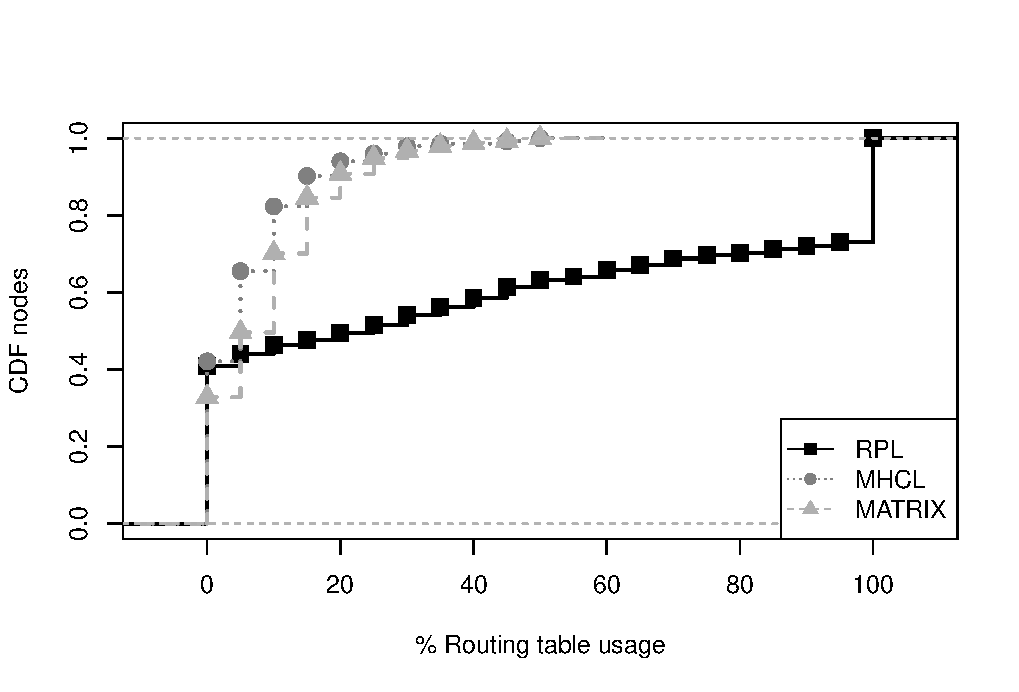
\includegraphics[width=0.95\linewidth]{Images/tableentries.pdf}
    \caption{Routing table usage CDF. (Maximum table size = 20)}
    \label{fig:table-usage}
\end{figure}

Figure \ref{fig:beacons} illustrates the amount of control traffic
in our experiments (the total number of beacons sent during the entire
simulation).
Matrix sends fewer control packet than RPL, because it
only sends additional beacons during network initialization and in
case of collection tree topology updates, whereas RPL has a communication
intensive maintenance of downward routes during the entire execution time. 

\begin{figure}[h]
    \centering
    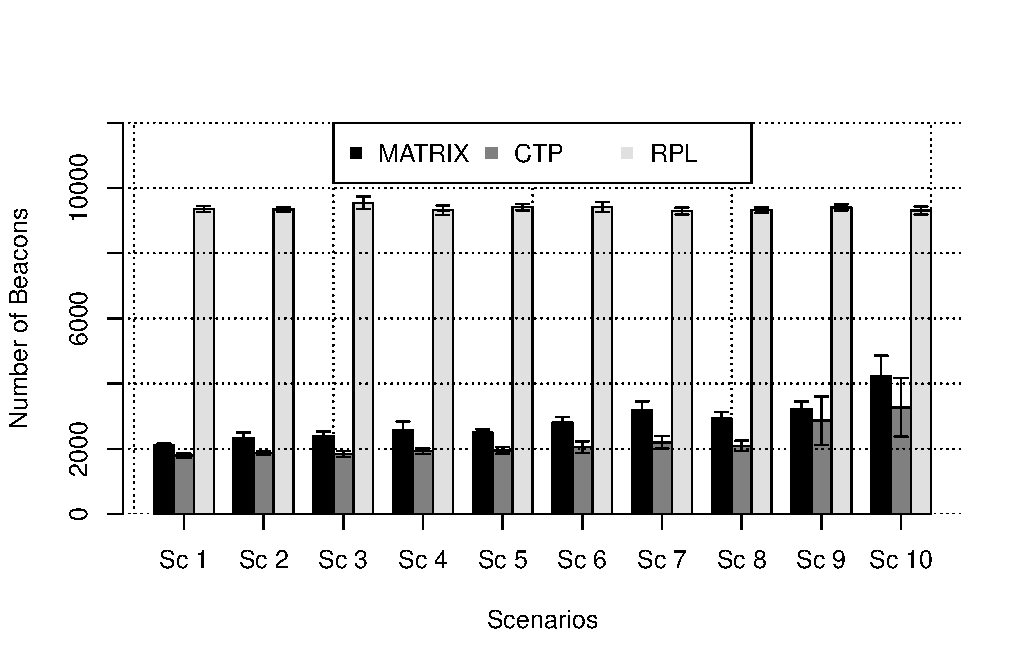
\includegraphics[width=0.95\linewidth]{Images/beacons.pdf}
    \caption{Number of control packets.}
    \label{fig:beacons}
\end{figure}

Figure~\ref{fig:footprint} compares RAM and ROM footprints in
the protocol stack of CTP, RPL and Matrix. We can see that Matrix adds only a
little more than 7KB of code to CTP, allowing this protocol to perform any-to-any communication with
high scalability. When compared with RPL, the execution code of
Matrix requires less RAM.
\begin{figure}[h]
    \centering
    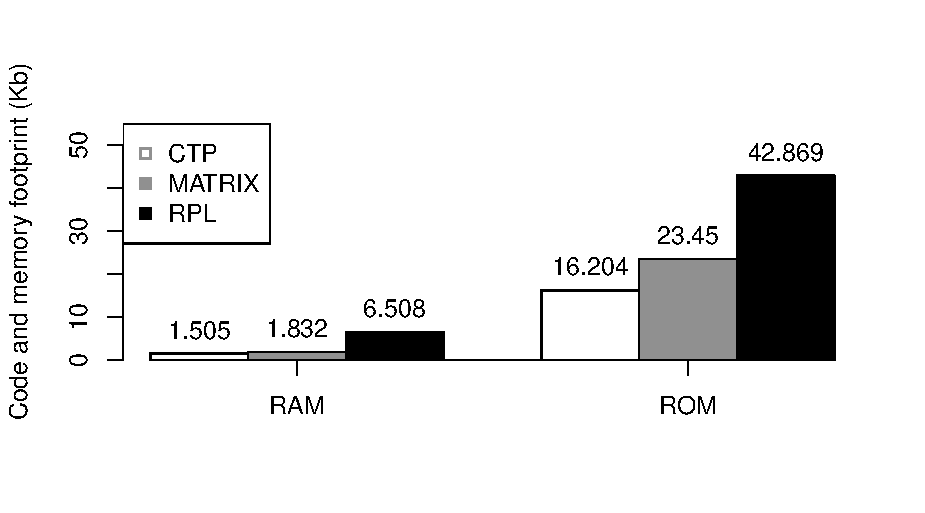
\includegraphics[width=0.82\linewidth]{Images/footprint.pdf}
    \caption{Code and memory footprint in bytes.}
    \label{fig:footprint}
\end{figure}

Our main result is illustrated in Figure~\ref{fig:txdwn}, which compares
top-down routing success rate. We measured the total
number of application (ack) messages sent downwards and successfully received by
the destination.\footnote{We do not plot the success rate of bottom-up traffic,
since it is done by the underlying collection protocol, without any intervention from Matrix
.} In the plot, ``inevitable losses'' refers to the
number of messages that were lost due to a failure of the destination node, in which case, there were no
valid path to the destination and the packet loss was inevitable.
The remaining messages were lost due to wireless collisions and node failures on
the packet's path. 

We can see that, when a valid path exists to the destination, the top-down
success rate of Matrix varies between 95\% and 99\%. In the harshest
faulty scenario 10,
without the local broadcast mechanism, MHCL delivers 85\% of top-down messages.
With the local broadcast activated, the success rate increases to 95\%,
i.e., roughly 2/3 of otherwise lost messages succeed in reaching the final
destination.
RPL, on the other hand, delivered less than $20\%$ of messages in all simulated
scenarios, which occurs due to lack of memory to store all the top-down routes.

\begin{figure}[h]
    \centering
    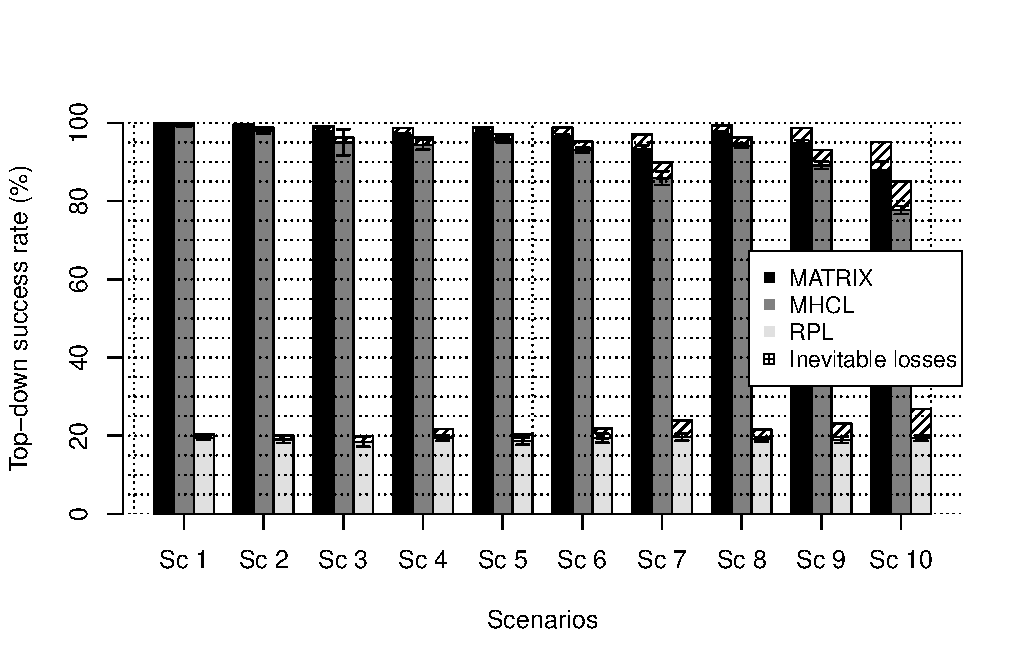
\includegraphics[width=1\linewidth]{Images/txrouting.pdf}
    \caption{Top-down routing success rate.}
    \label{fig:txdwn}
\end{figure}

\section{Related Work}
\label{sec:related}

AODV\cite{perkins2003ad} and DSR\cite{johnson2007rfc} are
traditional wireless protocols that allow any-to-any communication,
but they were designed for 802.11 and require too many states or
apply several overheads on the packet header.
%Our approach differ from traditional routing protocols by enabling any-to-any routes with low cost of states and overheads, also MATRIX provides by default IPv6 address allocation.
In the context of low-power and lossy networks, CTP\cite{Fonseca:2009} and
CodeDrip\cite{junior2014codedrip} were designed for bottom-up and
top-down data flows, respectively. They support communication in only one
direction.

State-of-the-art routing protocols for 6lowPAN that enable
any-to-any communication are RPL\cite{rfc6550}, XCTP\cite{xctp}, and
Hydro\cite{hydro}. RPL allows two modes of operation (storing and
non-storing) for downwards data flows. The non-storing mode is based
on source routing, and the storing mode pro-actively maintains an
entry in the routing table of every node on the path from the root
to each destination, which is not scalable to even moderate-size
networks. XCTP is an extension of CTP and is based on a reactive
reverse collection route creating between the root and every source
node. An entry in the reverse-route table is kept for every data
flow at each node on the path between the source and the
destination, which is also not scalable in terms of memory
footprint. Hydro protocol, like RPL, is based on a DAG
(directed acyclic graph) for bottom-up communication. Source nodes
need to periodically send reports to the border router, which builds
a global view (typically incomplete) of the network topology.

Some more recent protocols \cite{Palani2015, Moghadam:2015:MMR:2766739.2766774,
7374975} modified RPL to include new features. In~\cite{Palani2015}, a
load-balance technique is applied over nodes to decrease power consumption. In
\cite{Moghadam:2015:MMR:2766739.2766774, 7374975}, they provide multi-path
routing protocols to improve throughput and fault tolerance.

Matrix differs from previous work by providing a reliable and scalable solution
for any-to-any routing in 6LoWLAN, both in terms of routing table size and
control message overhead. Moreover, it allocates global and structured IPv6
addresses to all nodes, which allow nodes to act as destinations integrated into
the Internet, contributing to the realization of the Internet of Things.
\section*{Acknowledgments}
This work was supported in part by CAPES, CNPq and FAPEMIG.
\section{Conclusions}
\label{sec:conclusions}

In this work, we presented $\mu$Matrix: a memory efficient routing protocol for 6LoWPAN that performs any-to-any routing, hierarchical address allocation, and mobility management. As a building block of $\mu$Matrix, we proposed a passive mobility detection mechanism that captures topological changes without requiring additional hardware. Finally, we introduced the CRWP, a mobility model suited for scenarios with mobile nodes that have cyclical movement patterns. As future work, we plan to run experiments with physical devices and extend experimental evaluation to more mobile models, such as faulty communications scenarios. 

%
% The following two commands are all you need in the
% initial runs of your .tex file to
% produce the bibliography for the citations in your paper.

\bibliographystyle{elsarticle-num}

\bibliography{references}  % sigproc.bib is the name of the Bibliography in this case
% You must have a proper ".bib" file
%  and remember to run:
% latex bibtex latex latex
% to resolve all references
%
% ACM needs 'a single self-contained file'!
%
%APPENDICES are optional
%\balancecolumns
%\balancecolumns % GM June 2007
% That's all folks!
\end{document}
